\documentclass[1p]{elsarticle_modified}
%\bibliographystyle{elsarticle-num}

%\usepackage[colorlinks]{hyperref}
%\usepackage{abbrmath_seonhwa} %\Abb, \Ascr, \Acal ,\Abf, \Afrak
\usepackage{amsfonts}
\usepackage{amssymb}
\usepackage{amsmath}
\usepackage{amsthm}
\usepackage{scalefnt}
\usepackage{amsbsy}
\usepackage{kotex}
\usepackage{caption}
\usepackage{subfig}
\usepackage{color}
\usepackage{graphicx}
\usepackage{xcolor} %% white, black, red, green, blue, cyan, magenta, yellow
\usepackage{float}
\usepackage{setspace}
\usepackage{hyperref}

\usepackage{tikz}
\usetikzlibrary{arrows}

\usepackage{multirow}
\usepackage{array} % fixed length table
\usepackage{hhline}

%%%%%%%%%%%%%%%%%%%%%
\makeatletter
\renewcommand*\env@matrix[1][\arraystretch]{%
	\edef\arraystretch{#1}%
	\hskip -\arraycolsep
	\let\@ifnextchar\new@ifnextchar
	\array{*\c@MaxMatrixCols c}}
\makeatother %https://tex.stackexchange.com/questions/14071/how-can-i-increase-the-line-spacing-in-a-matrix
%%%%%%%%%%%%%%%

\usepackage[normalem]{ulem}

\newcommand{\msout}[1]{\ifmmode\text{\sout{\ensuremath{#1}}}\else\sout{#1}\fi}
%SOURCE: \msout is \stkout macro in https://tex.stackexchange.com/questions/20609/strikeout-in-math-mode

\newcommand{\cancel}[1]{
	\ifmmode
	{\color{red}\msout{#1}}
	\else
	{\color{red}\sout{#1}}
	\fi
}

\newcommand{\add}[1]{
	{\color{blue}\uwave{#1}}
}

\newcommand{\replace}[2]{
	\ifmmode
	{\color{red}\msout{#1}}{\color{blue}\uwave{#2}}
	\else
	{\color{red}\sout{#1}}{\color{blue}\uwave{#2}}
	\fi
}

\newcommand{\Sol}{\mathcal{S}} %segment
\newcommand{\D}{D} %diagram
\newcommand{\A}{\mathcal{A}} %arc


%%%%%%%%%%%%%%%%%%%%%%%%%%%%%5 test

\def\sl{\operatorname{\textup{SL}}(2,\Cbb)}
\def\psl{\operatorname{\textup{PSL}}(2,\Cbb)}
\def\quan{\mkern 1mu \triangleright \mkern 1mu}

\theoremstyle{definition}
\newtheorem{thm}{Theorem}[section]
\newtheorem{prop}[thm]{Proposition}
\newtheorem{lem}[thm]{Lemma}
\newtheorem{ques}[thm]{Question}
\newtheorem{cor}[thm]{Corollary}
\newtheorem{defn}[thm]{Definition}
\newtheorem{exam}[thm]{Example}
\newtheorem{rmk}[thm]{Remark}
\newtheorem{alg}[thm]{Algorithm}

\newcommand{\I}{\sqrt{-1}}
\begin{document}

%\begin{frontmatter}
%
%\title{Boundary parabolic representations of knots up to 8 crossings}
%
%%% Group authors per affiliation:
%\author{Yunhi Cho} 
%\address{Department of Mathematics, University of Seoul, Seoul, Korea}
%\ead{yhcho@uos.ac.kr}
%
%
%\author{Seonhwa Kim} %\fnref{s_kim}}
%\address{Center for Geometry and Physics, Institute for Basic Science, Pohang, 37673, Korea}
%\ead{ryeona17@ibs.re.kr}
%
%\author{Hyuk Kim}
%\address{Department of Mathematical Sciences, Seoul National University, Seoul 08826, Korea}
%\ead{hyukkim@snu.ac.kr}
%
%\author{Seokbeom Yoon}
%\address{Department of Mathematical Sciences, Seoul National University, Seoul, 08826,  Korea}
%\ead{sbyoon15@snu.ac.kr}
%
%\begin{abstract}
%We find all boundary parabolic representation of knots up to 8 crossings.
%
%\end{abstract}
%\begin{keyword}
%    \MSC[2010] 57M25 
%\end{keyword}
%
%\end{frontmatter}

%\linenumbers
%\tableofcontents
%
\newcommand\colored[1]{\textcolor{white}{\rule[-0.35ex]{0.8em}{1.4ex}}\kern-0.8em\color{red} #1}%
%\newcommand\colored[1]{\textcolor{white}{ #1}\kern-2.17ex	\textcolor{white}{ #1}\kern-1.81ex	\textcolor{white}{ #1}\kern-2.15ex\color{red}#1	}

{\Large $\underline{12a_{0707}~(K12a_{0707})}$}

\setlength{\tabcolsep}{10pt}
\renewcommand{\arraystretch}{1.6}
\vspace{1cm}\begin{tabular}{m{100pt}>{\centering\arraybackslash}m{274pt}}
\multirow{5}{120pt}{
	\centering
	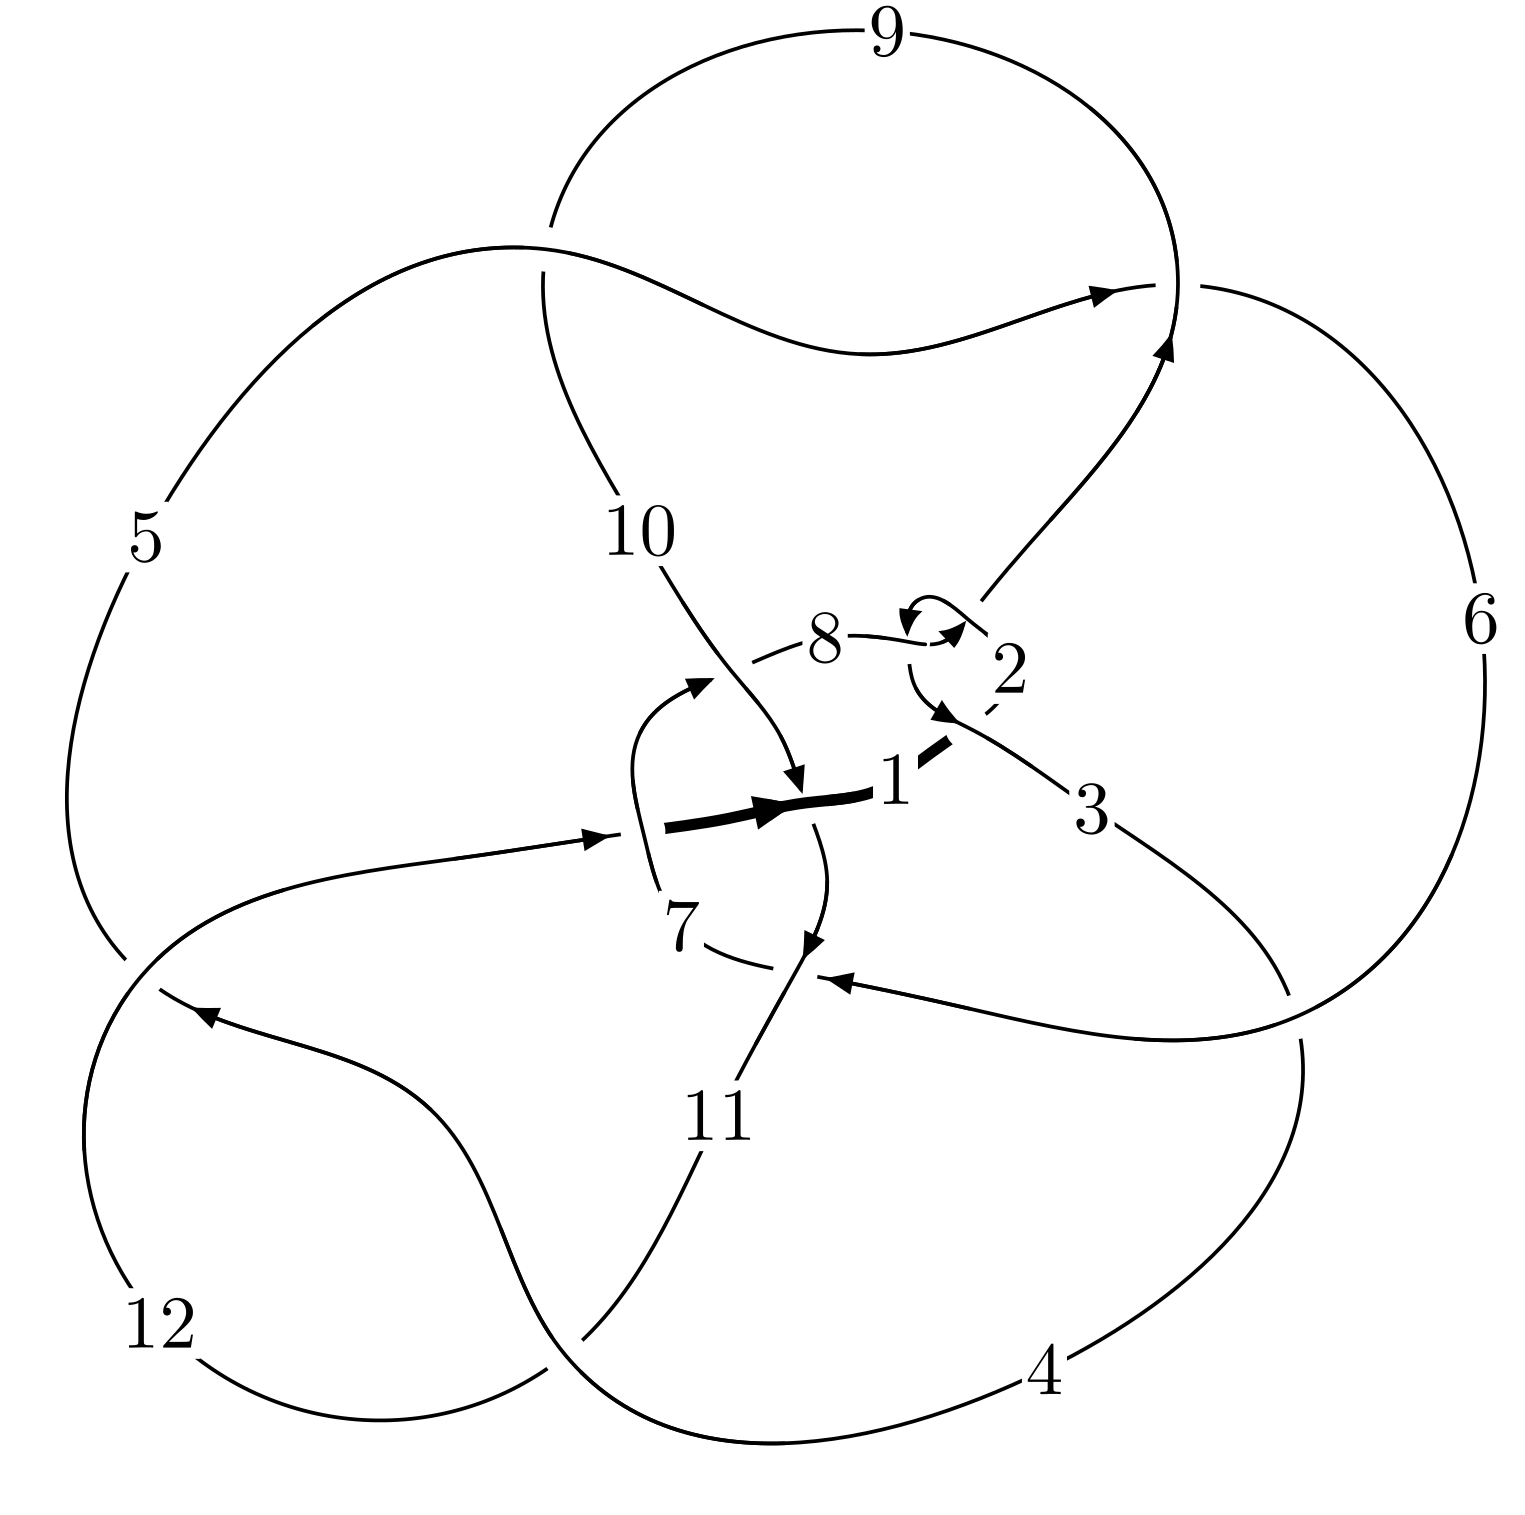
\includegraphics[width=112pt]{../../../GIT/diagram.site/Diagrams/png/1508_12a_0707.png}\\
\ \ \ A knot diagram\footnotemark}&
\allowdisplaybreaks
\textbf{Linearized knot diagam} \\
\cline{2-2}
 &
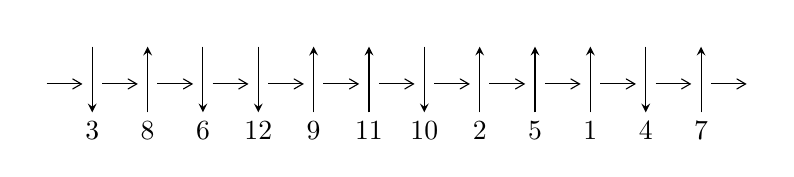
\begin{tikzpicture}[x=20pt, y=17pt]
	% nodes
	\node (C0) at (0, 0) {};
	\node (C1) at (1, 0) {};
	\node (C1U) at (1, +1) {};
	\node (C1D) at (1, -1) {3};

	\node (C2) at (2, 0) {};
	\node (C2U) at (2, +1) {};
	\node (C2D) at (2, -1) {8};

	\node (C3) at (3, 0) {};
	\node (C3U) at (3, +1) {};
	\node (C3D) at (3, -1) {6};

	\node (C4) at (4, 0) {};
	\node (C4U) at (4, +1) {};
	\node (C4D) at (4, -1) {12};

	\node (C5) at (5, 0) {};
	\node (C5U) at (5, +1) {};
	\node (C5D) at (5, -1) {9};

	\node (C6) at (6, 0) {};
	\node (C6U) at (6, +1) {};
	\node (C6D) at (6, -1) {11};

	\node (C7) at (7, 0) {};
	\node (C7U) at (7, +1) {};
	\node (C7D) at (7, -1) {10};

	\node (C8) at (8, 0) {};
	\node (C8U) at (8, +1) {};
	\node (C8D) at (8, -1) {2};

	\node (C9) at (9, 0) {};
	\node (C9U) at (9, +1) {};
	\node (C9D) at (9, -1) {5};

	\node (C10) at (10, 0) {};
	\node (C10U) at (10, +1) {};
	\node (C10D) at (10, -1) {1};

	\node (C11) at (11, 0) {};
	\node (C11U) at (11, +1) {};
	\node (C11D) at (11, -1) {4};

	\node (C12) at (12, 0) {};
	\node (C12U) at (12, +1) {};
	\node (C12D) at (12, -1) {7};
	\node (C13) at (13, 0) {};

	% arrows
	\draw[->,>={angle 60}]
	(C0) edge (C1) (C1) edge (C2) (C2) edge (C3) (C3) edge (C4) (C4) edge (C5) (C5) edge (C6) (C6) edge (C7) (C7) edge (C8) (C8) edge (C9) (C9) edge (C10) (C10) edge (C11) (C11) edge (C12) (C12) edge (C13) ;	\draw[->,>=stealth]
	(C1U) edge (C1D) (C2D) edge (C2U) (C3U) edge (C3D) (C4U) edge (C4D) (C5D) edge (C5U) (C6D) edge (C6U) (C7U) edge (C7D) (C8D) edge (C8U) (C9D) edge (C9U) (C10D) edge (C10U) (C11U) edge (C11D) (C12D) edge (C12U) ;
	\end{tikzpicture} \\
\hhline{~~} \\& 
\textbf{Solving Sequence} \\ \cline{2-2} 
 &
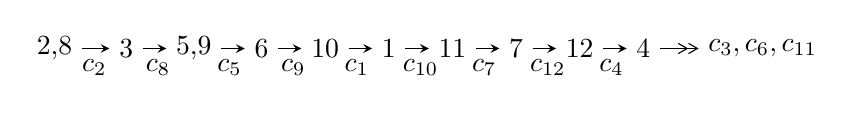
\begin{tikzpicture}[x=23pt, y=7pt]
	% node
	\node (A0) at (-1/8, 0) {2,8};
	\node (A1) at (1, 0) {3};
	\node (A2) at (33/16, 0) {5,9};
	\node (A3) at (25/8, 0) {6};
	\node (A4) at (33/8, 0) {10};
	\node (A5) at (41/8, 0) {1};
	\node (A6) at (49/8, 0) {11};
	\node (A7) at (57/8, 0) {7};
	\node (A8) at (65/8, 0) {12};
	\node (A9) at (73/8, 0) {4};
	\node (C1) at (1/2, -1) {$c_{2}$};
	\node (C2) at (3/2, -1) {$c_{8}$};
	\node (C3) at (21/8, -1) {$c_{5}$};
	\node (C4) at (29/8, -1) {$c_{9}$};
	\node (C5) at (37/8, -1) {$c_{1}$};
	\node (C6) at (45/8, -1) {$c_{10}$};
	\node (C7) at (53/8, -1) {$c_{7}$};
	\node (C8) at (61/8, -1) {$c_{12}$};
	\node (C9) at (69/8, -1) {$c_{4}$};
	\node (A10) at (11, 0) {$c_{3},c_{6},c_{11}$};

	% edge
	\draw[->,>=stealth]	
	(A0) edge (A1) (A1) edge (A2) (A2) edge (A3) (A3) edge (A4) (A4) edge (A5) (A5) edge (A6) (A6) edge (A7) (A7) edge (A8) (A8) edge (A9) ;
	\draw[->>,>={angle 60}]	
	(A9) edge (A10);
\end{tikzpicture} \\ 

\end{tabular} \\

\footnotetext{
The image of knot diagram is generated by the software ``\textbf{Draw programme}" developed by Andrew Bartholomew(\url{http://www.layer8.co.uk/maths/draw/index.htm\#Running-draw}), where we modified some parts for our purpose(\url{https://github.com/CATsTAILs/LinksPainter}).
}\phantom \\ \newline 
\centering \textbf{Ideals for irreducible components\footnotemark of $X_{\text{par}}$} 
 
\begin{align*}
I^u_{1}&=\langle 
1.86827\times10^{582} u^{181}-3.19856\times10^{582} u^{180}+\cdots+4.55306\times10^{582} b-5.56258\times10^{584},\\
\phantom{I^u_{1}}&\phantom{= \langle  }8.53302\times10^{584} u^{181}-1.42871\times10^{585} u^{180}+\cdots+2.94583\times10^{585} a-7.55853\times10^{586},\\
\phantom{I^u_{1}}&\phantom{= \langle  }u^{182}-2 u^{181}+\cdots-3170 u+647\rangle \\
I^u_{2}&=\langle 
1.43964\times10^{20} u^{47}-1.21238\times10^{20} u^{46}+\cdots+6.08163\times10^{19} b-2.83566\times10^{20},\\
\phantom{I^u_{2}}&\phantom{= \langle  }-1.37210\times10^{20} u^{47}-1.58559\times10^{20} u^{46}+\cdots+6.08163\times10^{19} a+2.09575\times10^{18},\;u^{48}+u^{47}+\cdots-3 u+1\rangle \\
\\
\end{align*}
\raggedright * 2 irreducible components of $\dim_{\mathbb{C}}=0$, with total 230 representations.\\
\footnotetext{All coefficients of polynomials are rational numbers. But the coefficients are sometimes approximated in decimal forms when there is not enough margin.}
\newpage
\renewcommand{\arraystretch}{1}
\centering \section*{I. $I^u_{1}= \langle 1.87\times10^{582} u^{181}-3.20\times10^{582} u^{180}+\cdots+4.55\times10^{582} b-5.56\times10^{584},\;8.53\times10^{584} u^{181}-1.43\times10^{585} u^{180}+\cdots+2.95\times10^{585} a-7.56\times10^{586},\;u^{182}-2 u^{181}+\cdots-3170 u+647 \rangle$}
\flushleft \textbf{(i) Arc colorings}\\
\begin{tabular}{m{7pt} m{180pt} m{7pt} m{180pt} }
\flushright $a_{2}=$&$\begin{pmatrix}1\\0\end{pmatrix}$ \\
\flushright $a_{8}=$&$\begin{pmatrix}0\\u\end{pmatrix}$ \\
\flushright $a_{3}=$&$\begin{pmatrix}1\\- u^2\end{pmatrix}$ \\
\flushright $a_{5}=$&$\begin{pmatrix}-0.289665 u^{181}+0.484993 u^{180}+\cdots-329.497 u+25.6584\\-0.410334 u^{181}+0.702509 u^{180}+\cdots-786.078 u+122.172\end{pmatrix}$ \\
\flushright $a_{9}=$&$\begin{pmatrix}u\\u\end{pmatrix}$ \\
\flushright $a_{6}=$&$\begin{pmatrix}-0.205771 u^{181}+0.418521 u^{180}+\cdots-326.941 u+41.0715\\-0.326440 u^{181}+0.636037 u^{180}+\cdots-783.522 u+137.586\end{pmatrix}$ \\
\flushright $a_{10}=$&$\begin{pmatrix}-0.197935 u^{181}+0.138456 u^{180}+\cdots+70.3475 u-47.6382\\-0.147855 u^{181}-0.0420209 u^{180}+\cdots+536.279 u-159.236\end{pmatrix}$ \\
\flushright $a_{1}=$&$\begin{pmatrix}u^2+1\\- u^4\end{pmatrix}$ \\
\flushright $a_{11}=$&$\begin{pmatrix}-0.332327 u^{181}+0.333486 u^{180}+\cdots-87.4336 u-38.9923\\-0.298887 u^{181}+0.266562 u^{180}+\cdots+160.525 u-94.6823\end{pmatrix}$ \\
\flushright $a_{7}=$&$\begin{pmatrix}-0.0325621 u^{181}-0.0922697 u^{180}+\cdots+468.771 u-103.076\\-0.171974 u^{181}+0.0272787 u^{180}+\cdots+596.604 u-166.450\end{pmatrix}$ \\
\flushright $a_{12}=$&$\begin{pmatrix}0.205787 u^{181}-0.713579 u^{180}+\cdots+1510.06 u-324.131\\0.164662 u^{181}-0.687047 u^{180}+\cdots+1411.00 u-302.943\end{pmatrix}$ \\
\flushright $a_{4}=$&$\begin{pmatrix}-0.472037 u^{181}+1.14659 u^{180}+\cdots-1749.16 u+331.262\\-0.405221 u^{181}+1.17867 u^{180}+\cdots-2092.49 u+429.490\end{pmatrix}$\\&\end{tabular}
\flushleft \textbf{(ii) Obstruction class $= -1$}\\~\\
\flushleft \textbf{(iii) Cusp Shapes $= 0.486313 u^{181}-0.0903998 u^{180}+\cdots-1349.49 u+429.270$}\\~\\
\newpage\renewcommand{\arraystretch}{1}
\flushleft \textbf{(iv) u-Polynomials at the component}\newline \\
\begin{tabular}{m{50pt}|m{274pt}}
Crossings & \hspace{64pt}u-Polynomials at each crossing \\
\hline $$\begin{aligned}c_{1}\end{aligned}$$&$\begin{aligned}
&u^{182}+88 u^{181}+\cdots+9154060 u+418609
\end{aligned}$\\
\hline $$\begin{aligned}c_{2},c_{8}\end{aligned}$$&$\begin{aligned}
&u^{182}+2 u^{181}+\cdots+3170 u+647
\end{aligned}$\\
\hline $$\begin{aligned}c_{3}\end{aligned}$$&$\begin{aligned}
&u^{182}-9 u^{181}+\cdots-4473834946 u+318667011
\end{aligned}$\\
\hline $$\begin{aligned}c_{4},c_{11}\end{aligned}$$&$\begin{aligned}
&u^{182}-65 u^{180}+\cdots+17454 u+6196
\end{aligned}$\\
\hline $$\begin{aligned}c_{5},c_{9}\end{aligned}$$&$\begin{aligned}
&u^{182}+48 u^{180}+\cdots+935357 u+53761
\end{aligned}$\\
\hline $$\begin{aligned}c_{6}\end{aligned}$$&$\begin{aligned}
&u^{182}-3 u^{181}+\cdots+4259486 u+3695609
\end{aligned}$\\
\hline $$\begin{aligned}c_{7}\end{aligned}$$&$\begin{aligned}
&u^{182}-9 u^{181}+\cdots-7454 u+3031
\end{aligned}$\\
\hline $$\begin{aligned}c_{10}\end{aligned}$$&$\begin{aligned}
&u^{182}+28 u^{181}+\cdots+9541 u+457
\end{aligned}$\\
\hline $$\begin{aligned}c_{12}\end{aligned}$$&$\begin{aligned}
&u^{182}+u^{181}+\cdots+10 u+3
\end{aligned}$\\
\hline
\end{tabular}\\~\\
\newpage\renewcommand{\arraystretch}{1}
\flushleft \textbf{(v) Riley Polynomials at the component}\newline \\
\begin{tabular}{m{50pt}|m{274pt}}
Crossings & \hspace{64pt}Riley Polynomials at each crossing \\
\hline $$\begin{aligned}c_{1}\end{aligned}$$&$\begin{aligned}
&y^{182}+28 y^{181}+\cdots+3612930806400 y+175233494881
\end{aligned}$\\
\hline $$\begin{aligned}c_{2},c_{8}\end{aligned}$$&$\begin{aligned}
&y^{182}+88 y^{181}+\cdots+9154060 y+418609
\end{aligned}$\\
\hline $$\begin{aligned}c_{3}\end{aligned}$$&$\begin{aligned}
&y^{182}-49 y^{181}+\cdots+2.91\times10^{18} y+1.02\times10^{17}
\end{aligned}$\\
\hline $$\begin{aligned}c_{4},c_{11}\end{aligned}$$&$\begin{aligned}
&y^{182}-130 y^{181}+\cdots-1577213772 y+38390416
\end{aligned}$\\
\hline $$\begin{aligned}c_{5},c_{9}\end{aligned}$$&$\begin{aligned}
&y^{182}+96 y^{181}+\cdots+152047431545 y+2890245121
\end{aligned}$\\
\hline $$\begin{aligned}c_{6}\end{aligned}$$&$\begin{aligned}
&y^{182}+27 y^{181}+\cdots+3313957547436004 y+13657525880881
\end{aligned}$\\
\hline $$\begin{aligned}c_{7}\end{aligned}$$&$\begin{aligned}
&y^{182}-7 y^{181}+\cdots+874676032 y+9186961
\end{aligned}$\\
\hline $$\begin{aligned}c_{10}\end{aligned}$$&$\begin{aligned}
&y^{182}-6 y^{181}+\cdots+15585591 y+208849
\end{aligned}$\\
\hline $$\begin{aligned}c_{12}\end{aligned}$$&$\begin{aligned}
&y^{182}+25 y^{181}+\cdots-508 y+9
\end{aligned}$\\
\hline
\end{tabular}\\~\\
\newpage\flushleft \textbf{(vi) Complex Volumes and Cusp Shapes}
$$\begin{array}{c|c|c}  
\text{Solutions to }I^u_{1}& \I (\text{vol} + \sqrt{-1}CS) & \text{Cusp shape}\\
 \hline 
\begin{aligned}
u &= -0.256529 + 0.965217 I \\
a &= \phantom{-}1.212430 - 0.659498 I \\
b &= \phantom{-}1.004440 - 0.357173 I\end{aligned}
 & -1.93206 - 2.87680 I & \phantom{-0.000000 } 0 \\ \hline\begin{aligned}
u &= -0.256529 - 0.965217 I \\
a &= \phantom{-}1.212430 + 0.659498 I \\
b &= \phantom{-}1.004440 + 0.357173 I\end{aligned}
 & -1.93206 + 2.87680 I & \phantom{-0.000000 } 0 \\ \hline\begin{aligned}
u &= \phantom{-}0.321283 + 0.960383 I \\
a &= -1.72160 - 1.88464 I \\
b &= -1.42332 - 1.65390 I\end{aligned}
 & -4.04300 + 7.35745 I & \phantom{-0.000000 } 0 \\ \hline\begin{aligned}
u &= \phantom{-}0.321283 - 0.960383 I \\
a &= -1.72160 + 1.88464 I \\
b &= -1.42332 + 1.65390 I\end{aligned}
 & -4.04300 - 7.35745 I & \phantom{-0.000000 } 0 \\ \hline\begin{aligned}
u &= -0.959093 + 0.342048 I \\
a &= -0.11658 - 1.83837 I \\
b &= -0.017897 - 0.543037 I\end{aligned}
 & \phantom{-}0.04523 + 8.72598 I & \phantom{-0.000000 } 0 \\ \hline\begin{aligned}
u &= -0.959093 - 0.342048 I \\
a &= -0.11658 + 1.83837 I \\
b &= -0.017897 + 0.543037 I\end{aligned}
 & \phantom{-}0.04523 - 8.72598 I & \phantom{-0.000000 } 0 \\ \hline\begin{aligned}
u &= \phantom{-}0.970839 + 0.334543 I \\
a &= \phantom{-}0.11427 - 1.61623 I \\
b &= \phantom{-}0.214960 - 0.356312 I\end{aligned}
 & -5.85337 - 2.71377 I & \phantom{-0.000000 } 0 \\ \hline\begin{aligned}
u &= \phantom{-}0.970839 - 0.334543 I \\
a &= \phantom{-}0.11427 + 1.61623 I \\
b &= \phantom{-}0.214960 + 0.356312 I\end{aligned}
 & -5.85337 + 2.71377 I & \phantom{-0.000000 } 0 \\ \hline\begin{aligned}
u &= \phantom{-}0.319026 + 0.917578 I \\
a &= \phantom{-}3.14081 + 0.70461 I \\
b &= \phantom{-}3.91127 + 1.02720 I\end{aligned}
 & -3.90447 - 4.81068 I & \phantom{-0.000000 } 0 \\ \hline\begin{aligned}
u &= \phantom{-}0.319026 - 0.917578 I \\
a &= \phantom{-}3.14081 - 0.70461 I \\
b &= \phantom{-}3.91127 - 1.02720 I\end{aligned}
 & -3.90447 + 4.81068 I & \phantom{-0.000000 } 0\\
 \hline 
 \end{array}$$\newpage$$\begin{array}{c|c|c}  
\text{Solutions to }I^u_{1}& \I (\text{vol} + \sqrt{-1}CS) & \text{Cusp shape}\\
 \hline 
\begin{aligned}
u &= \phantom{-}0.963066 + 0.370945 I \\
a &= -0.00320 - 1.87437 I \\
b &= -0.131414 - 0.487661 I\end{aligned}
 & -3.8848 - 15.0556 I & \phantom{-0.000000 } 0 \\ \hline\begin{aligned}
u &= \phantom{-}0.963066 - 0.370945 I \\
a &= -0.00320 + 1.87437 I \\
b &= -0.131414 + 0.487661 I\end{aligned}
 & -3.8848 + 15.0556 I & \phantom{-0.000000 } 0 \\ \hline\begin{aligned}
u &= -0.215480 + 1.011660 I \\
a &= -0.95136 - 1.10794 I \\
b &= -2.30367 - 0.96336 I\end{aligned}
 & -8.52535 - 5.59306 I & \phantom{-0.000000 } 0 \\ \hline\begin{aligned}
u &= -0.215480 - 1.011660 I \\
a &= -0.95136 + 1.10794 I \\
b &= -2.30367 + 0.96336 I\end{aligned}
 & -8.52535 + 5.59306 I & \phantom{-0.000000 } 0 \\ \hline\begin{aligned}
u &= \phantom{-}0.416754 + 0.947098 I \\
a &= -1.84060 - 0.40313 I \\
b &= -2.99579 - 0.35572 I\end{aligned}
 & -2.45544 + 6.04571 I & \phantom{-0.000000 } 0 \\ \hline\begin{aligned}
u &= \phantom{-}0.416754 - 0.947098 I \\
a &= -1.84060 + 0.40313 I \\
b &= -2.99579 + 0.35572 I\end{aligned}
 & -2.45544 - 6.04571 I & \phantom{-0.000000 } 0 \\ \hline\begin{aligned}
u &= -0.408551 + 0.952318 I \\
a &= \phantom{-}0.141264 + 0.895448 I \\
b &= \phantom{-}0.959008 - 0.391747 I\end{aligned}
 & -2.83544 - 2.47905 I & \phantom{-0.000000 } 0 \\ \hline\begin{aligned}
u &= -0.408551 - 0.952318 I \\
a &= \phantom{-}0.141264 - 0.895448 I \\
b &= \phantom{-}0.959008 + 0.391747 I\end{aligned}
 & -2.83544 + 2.47905 I & \phantom{-0.000000 } 0 \\ \hline\begin{aligned}
u &= \phantom{-}0.755664 + 0.592081 I \\
a &= \phantom{-}0.44078 + 2.25804 I \\
b &= \phantom{-}0.232245 + 1.140070 I\end{aligned}
 & -0.20565 - 5.15931 I & \phantom{-0.000000 } 0 \\ \hline\begin{aligned}
u &= \phantom{-}0.755664 - 0.592081 I \\
a &= \phantom{-}0.44078 - 2.25804 I \\
b &= \phantom{-}0.232245 - 1.140070 I\end{aligned}
 & -0.20565 + 5.15931 I & \phantom{-0.000000 } 0\\
 \hline 
 \end{array}$$\newpage$$\begin{array}{c|c|c}  
\text{Solutions to }I^u_{1}& \I (\text{vol} + \sqrt{-1}CS) & \text{Cusp shape}\\
 \hline 
\begin{aligned}
u &= -0.368804 + 0.974258 I \\
a &= -2.05082 + 1.21378 I \\
b &= -2.96000 + 1.39186 I\end{aligned}
 & -2.49284 + 0.44505 I & \phantom{-0.000000 } 0 \\ \hline\begin{aligned}
u &= -0.368804 - 0.974258 I \\
a &= -2.05082 - 1.21378 I \\
b &= -2.96000 - 1.39186 I\end{aligned}
 & -2.49284 - 0.44505 I & \phantom{-0.000000 } 0 \\ \hline\begin{aligned}
u &= -0.333309 + 0.990772 I \\
a &= -1.71075 - 1.18845 I \\
b &= -2.97767 - 0.52283 I\end{aligned}
 & -9.06733 + 3.65813 I & \phantom{-0.000000 } 0 \\ \hline\begin{aligned}
u &= -0.333309 - 0.990772 I \\
a &= -1.71075 + 1.18845 I \\
b &= -2.97767 + 0.52283 I\end{aligned}
 & -9.06733 - 3.65813 I & \phantom{-0.000000 } 0 \\ \hline\begin{aligned}
u &= \phantom{-}0.138390 + 0.932899 I \\
a &= -0.436637 - 0.107081 I \\
b &= -2.07183 - 0.66879 I\end{aligned}
 & -8.37172 - 5.25239 I & \phantom{-0.000000 } 0 \\ \hline\begin{aligned}
u &= \phantom{-}0.138390 - 0.932899 I \\
a &= -0.436637 + 0.107081 I \\
b &= -2.07183 + 0.66879 I\end{aligned}
 & -8.37172 + 5.25239 I & \phantom{-0.000000 } 0 \\ \hline\begin{aligned}
u &= -0.811952 + 0.684382 I \\
a &= \phantom{-}0.152594 + 0.455598 I \\
b &= -0.629575 + 0.558511 I\end{aligned}
 & \phantom{-}0.843620 + 0.857755 I & \phantom{-0.000000 } 0 \\ \hline\begin{aligned}
u &= -0.811952 - 0.684382 I \\
a &= \phantom{-}0.152594 - 0.455598 I \\
b &= -0.629575 - 0.558511 I\end{aligned}
 & \phantom{-}0.843620 - 0.857755 I & \phantom{-0.000000 } 0 \\ \hline\begin{aligned}
u &= \phantom{-}0.658901 + 0.834756 I \\
a &= -0.114461 + 0.485796 I \\
b &= \phantom{-}0.183497 - 0.212440 I\end{aligned}
 & \phantom{-}3.93302 + 0.52408 I & \phantom{-0.000000 } 0 \\ \hline\begin{aligned}
u &= \phantom{-}0.658901 - 0.834756 I \\
a &= -0.114461 - 0.485796 I \\
b &= \phantom{-}0.183497 + 0.212440 I\end{aligned}
 & \phantom{-}3.93302 - 0.52408 I & \phantom{-0.000000 } 0\\
 \hline 
 \end{array}$$\newpage$$\begin{array}{c|c|c}  
\text{Solutions to }I^u_{1}& \I (\text{vol} + \sqrt{-1}CS) & \text{Cusp shape}\\
 \hline 
\begin{aligned}
u &= -0.493093 + 0.962507 I \\
a &= -0.192912 + 0.349341 I \\
b &= -1.24572 - 1.46013 I\end{aligned}
 & -1.88389 - 2.60833 I & \phantom{-0.000000 } 0 \\ \hline\begin{aligned}
u &= -0.493093 - 0.962507 I \\
a &= -0.192912 - 0.349341 I \\
b &= -1.24572 + 1.46013 I\end{aligned}
 & -1.88389 + 2.60833 I & \phantom{-0.000000 } 0 \\ \hline\begin{aligned}
u &= \phantom{-}0.777088 + 0.489267 I \\
a &= -0.164620 - 1.363070 I \\
b &= -0.055748 + 0.181182 I\end{aligned}
 & -3.36835 - 6.51503 I & \phantom{-0.000000 } 0 \\ \hline\begin{aligned}
u &= \phantom{-}0.777088 - 0.489267 I \\
a &= -0.164620 + 1.363070 I \\
b &= -0.055748 - 0.181182 I\end{aligned}
 & -3.36835 + 6.51503 I & \phantom{-0.000000 } 0 \\ \hline\begin{aligned}
u &= -0.787498 + 0.461357 I \\
a &= -0.28773 - 1.49689 I \\
b &= -0.327748 - 0.486408 I\end{aligned}
 & \phantom{-}2.73572 - 0.70337 I & \phantom{-0.000000 } 0 \\ \hline\begin{aligned}
u &= -0.787498 - 0.461357 I \\
a &= -0.28773 + 1.49689 I \\
b &= -0.327748 + 0.486408 I\end{aligned}
 & \phantom{-}2.73572 + 0.70337 I & \phantom{-0.000000 } 0 \\ \hline\begin{aligned}
u &= \phantom{-}0.706324 + 0.828826 I \\
a &= -0.188825 + 0.116889 I \\
b &= -0.871915 + 0.357366 I\end{aligned}
 & \phantom{-}3.96907 + 4.70193 I & \phantom{-0.000000 } 0 \\ \hline\begin{aligned}
u &= \phantom{-}0.706324 - 0.828826 I \\
a &= -0.188825 - 0.116889 I \\
b &= -0.871915 - 0.357366 I\end{aligned}
 & \phantom{-}3.96907 - 4.70193 I & \phantom{-0.000000 } 0 \\ \hline\begin{aligned}
u &= \phantom{-}0.325079 + 1.041610 I \\
a &= \phantom{-}1.36015 - 0.95861 I \\
b &= \phantom{-}2.43676 - 0.48875 I\end{aligned}
 & -5.32911 + 0.68825 I & \phantom{-0.000000 } 0 \\ \hline\begin{aligned}
u &= \phantom{-}0.325079 - 1.041610 I \\
a &= \phantom{-}1.36015 + 0.95861 I \\
b &= \phantom{-}2.43676 + 0.48875 I\end{aligned}
 & -5.32911 - 0.68825 I & \phantom{-0.000000 } 0\\
 \hline 
 \end{array}$$\newpage$$\begin{array}{c|c|c}  
\text{Solutions to }I^u_{1}& \I (\text{vol} + \sqrt{-1}CS) & \text{Cusp shape}\\
 \hline 
\begin{aligned}
u &= -0.191530 + 1.084320 I \\
a &= -0.823473 + 0.326919 I \\
b &= -0.810574 - 0.652656 I\end{aligned}
 & -5.37510 + 6.53386 I & \phantom{-0.000000 } 0 \\ \hline\begin{aligned}
u &= -0.191530 - 1.084320 I \\
a &= -0.823473 - 0.326919 I \\
b &= -0.810574 + 0.652656 I\end{aligned}
 & -5.37510 - 6.53386 I & \phantom{-0.000000 } 0 \\ \hline\begin{aligned}
u &= \phantom{-}0.719448 + 0.530043 I \\
a &= \phantom{-}0.52019 - 1.69968 I \\
b &= \phantom{-}0.417648 - 0.853260 I\end{aligned}
 & -0.02194 + 6.24473 I & \phantom{-0.000000 } 0 \\ \hline\begin{aligned}
u &= \phantom{-}0.719448 - 0.530043 I \\
a &= \phantom{-}0.52019 + 1.69968 I \\
b &= \phantom{-}0.417648 + 0.853260 I\end{aligned}
 & -0.02194 - 6.24473 I & \phantom{-0.000000 } 0 \\ \hline\begin{aligned}
u &= -0.324042 + 0.829369 I \\
a &= \phantom{-}1.056160 - 0.040146 I \\
b &= \phantom{-}2.63404 - 0.02893 I\end{aligned}
 & -2.25972 - 0.64288 I & \phantom{-0.000000 } 0 \\ \hline\begin{aligned}
u &= -0.324042 - 0.829369 I \\
a &= \phantom{-}1.056160 + 0.040146 I \\
b &= \phantom{-}2.63404 + 0.02893 I\end{aligned}
 & -2.25972 + 0.64288 I & \phantom{-0.000000 } 0 \\ \hline\begin{aligned}
u &= \phantom{-}0.785872 + 0.786239 I \\
a &= -0.242549 + 0.418626 I \\
b &= \phantom{-}0.336274 + 0.888423 I\end{aligned}
 & \phantom{-}1.372790 - 0.122237 I & \phantom{-0.000000 } 0 \\ \hline\begin{aligned}
u &= \phantom{-}0.785872 - 0.786239 I \\
a &= -0.242549 - 0.418626 I \\
b &= \phantom{-}0.336274 - 0.888423 I\end{aligned}
 & \phantom{-}1.372790 + 0.122237 I & \phantom{-0.000000 } 0 \\ \hline\begin{aligned}
u &= \phantom{-}0.737790 + 0.492461 I \\
a &= \phantom{-}0.345930 + 0.026591 I \\
b &= -0.639912 + 0.349896 I\end{aligned}
 & \phantom{-}3.01770 - 3.51677 I & \phantom{-0.000000 } 0 \\ \hline\begin{aligned}
u &= \phantom{-}0.737790 - 0.492461 I \\
a &= \phantom{-}0.345930 - 0.026591 I \\
b &= -0.639912 - 0.349896 I\end{aligned}
 & \phantom{-}3.01770 + 3.51677 I & \phantom{-0.000000 } 0\\
 \hline 
 \end{array}$$\newpage$$\begin{array}{c|c|c}  
\text{Solutions to }I^u_{1}& \I (\text{vol} + \sqrt{-1}CS) & \text{Cusp shape}\\
 \hline 
\begin{aligned}
u &= -0.788821 + 0.390879 I \\
a &= -1.07972 + 1.10131 I \\
b &= -0.344559 + 0.168399 I\end{aligned}
 & -3.85365 - 3.48929 I & \phantom{-0.000000 } 0 \\ \hline\begin{aligned}
u &= -0.788821 - 0.390879 I \\
a &= -1.07972 - 1.10131 I \\
b &= -0.344559 - 0.168399 I\end{aligned}
 & -3.85365 + 3.48929 I & \phantom{-0.000000 } 0 \\ \hline\begin{aligned}
u &= -0.535493 + 0.990011 I \\
a &= -0.362014 + 0.582134 I \\
b &= -1.52400 + 0.09166 I\end{aligned}
 & -1.91170 - 3.00635 I & \phantom{-0.000000 } 0 \\ \hline\begin{aligned}
u &= -0.535493 - 0.990011 I \\
a &= -0.362014 - 0.582134 I \\
b &= -1.52400 - 0.09166 I\end{aligned}
 & -1.91170 + 3.00635 I & \phantom{-0.000000 } 0 \\ \hline\begin{aligned}
u &= \phantom{-}0.462803 + 1.029870 I \\
a &= -0.492012 + 0.113505 I \\
b &= -0.89362 + 1.44155 I\end{aligned}
 & \phantom{-}0.52559 + 3.16200 I & \phantom{-0.000000 } 0 \\ \hline\begin{aligned}
u &= \phantom{-}0.462803 - 1.029870 I \\
a &= -0.492012 - 0.113505 I \\
b &= -0.89362 - 1.44155 I\end{aligned}
 & \phantom{-}0.52559 - 3.16200 I & \phantom{-0.000000 } 0 \\ \hline\begin{aligned}
u &= -0.542683 + 0.990584 I \\
a &= \phantom{-}0.326897 + 0.168603 I \\
b &= \phantom{-}0.520159 + 1.250960 I\end{aligned}
 & \phantom{-}0.62605 - 2.30354 I & \phantom{-0.000000 } 0 \\ \hline\begin{aligned}
u &= -0.542683 - 0.990584 I \\
a &= \phantom{-}0.326897 - 0.168603 I \\
b &= \phantom{-}0.520159 - 1.250960 I\end{aligned}
 & \phantom{-}0.62605 + 2.30354 I & \phantom{-0.000000 } 0 \\ \hline\begin{aligned}
u &= -0.868493 + 0.017213 I \\
a &= -0.057365 - 1.337690 I \\
b &= -0.709355 - 0.117998 I\end{aligned}
 & -3.47721 - 2.37734 I & \phantom{-0.000000 } 0 \\ \hline\begin{aligned}
u &= -0.868493 - 0.017213 I \\
a &= -0.057365 + 1.337690 I \\
b &= -0.709355 + 0.117998 I\end{aligned}
 & -3.47721 + 2.37734 I & \phantom{-0.000000 } 0\\
 \hline 
 \end{array}$$\newpage$$\begin{array}{c|c|c}  
\text{Solutions to }I^u_{1}& \I (\text{vol} + \sqrt{-1}CS) & \text{Cusp shape}\\
 \hline 
\begin{aligned}
u &= \phantom{-}0.398745 + 1.063230 I \\
a &= -1.080680 + 0.294267 I \\
b &= -2.47122 - 0.39892 I\end{aligned}
 & -9.96700 + 7.36444 I & \phantom{-0.000000 } 0 \\ \hline\begin{aligned}
u &= \phantom{-}0.398745 - 1.063230 I \\
a &= -1.080680 - 0.294267 I \\
b &= -2.47122 + 0.39892 I\end{aligned}
 & -9.96700 - 7.36444 I & \phantom{-0.000000 } 0 \\ \hline\begin{aligned}
u &= \phantom{-}0.220809 + 1.117270 I \\
a &= \phantom{-}1.61693 - 0.13299 I \\
b &= \phantom{-}2.51781 + 0.37798 I\end{aligned}
 & -4.29846 - 1.07449 I & \phantom{-0.000000 } 0 \\ \hline\begin{aligned}
u &= \phantom{-}0.220809 - 1.117270 I \\
a &= \phantom{-}1.61693 + 0.13299 I \\
b &= \phantom{-}2.51781 - 0.37798 I\end{aligned}
 & -4.29846 + 1.07449 I & \phantom{-0.000000 } 0 \\ \hline\begin{aligned}
u &= \phantom{-}0.333221 + 0.791199 I \\
a &= \phantom{-}1.14122 + 1.43106 I \\
b &= \phantom{-}0.487291 + 0.418115 I\end{aligned}
 & -1.82793 - 2.81146 I & \phantom{-0.000000 } 0 \\ \hline\begin{aligned}
u &= \phantom{-}0.333221 - 0.791199 I \\
a &= \phantom{-}1.14122 - 1.43106 I \\
b &= \phantom{-}0.487291 - 0.418115 I\end{aligned}
 & -1.82793 + 2.81146 I & \phantom{-0.000000 } 0 \\ \hline\begin{aligned}
u &= -0.658819 + 0.549326 I \\
a &= \phantom{-}0.376897 - 0.103555 I \\
b &= -0.663931 + 0.009059 I\end{aligned}
 & \phantom{-}1.40731 - 1.37987 I & \phantom{-0.000000 } 0 \\ \hline\begin{aligned}
u &= -0.658819 - 0.549326 I \\
a &= \phantom{-}0.376897 + 0.103555 I \\
b &= -0.663931 - 0.009059 I\end{aligned}
 & \phantom{-}1.40731 + 1.37987 I & \phantom{-0.000000 } 0 \\ \hline\begin{aligned}
u &= -0.757703 + 0.401729 I \\
a &= -0.521099 - 0.085871 I \\
b &= \phantom{-}0.804581 + 0.237617 I\end{aligned}
 & -0.67887 + 8.76569 I & \phantom{-0.000000 } 0 \\ \hline\begin{aligned}
u &= -0.757703 - 0.401729 I \\
a &= -0.521099 + 0.085871 I \\
b &= \phantom{-}0.804581 - 0.237617 I\end{aligned}
 & -0.67887 - 8.76569 I & \phantom{-0.000000 } 0\\
 \hline 
 \end{array}$$\newpage$$\begin{array}{c|c|c}  
\text{Solutions to }I^u_{1}& \I (\text{vol} + \sqrt{-1}CS) & \text{Cusp shape}\\
 \hline 
\begin{aligned}
u &= \phantom{-}0.197885 + 1.127370 I \\
a &= \phantom{-}0.061092 - 0.496396 I \\
b &= \phantom{-}0.405840 + 0.174285 I\end{aligned}
 & -6.12079 + 0.96304 I & \phantom{-0.000000 } 0 \\ \hline\begin{aligned}
u &= \phantom{-}0.197885 - 1.127370 I \\
a &= \phantom{-}0.061092 + 0.496396 I \\
b &= \phantom{-}0.405840 - 0.174285 I\end{aligned}
 & -6.12079 - 0.96304 I & \phantom{-0.000000 } 0 \\ \hline\begin{aligned}
u &= \phantom{-}0.772578 + 0.355421 I \\
a &= \phantom{-}0.01052 + 2.03459 I \\
b &= \phantom{-}0.143729 + 0.599365 I\end{aligned}
 & \phantom{-}0.33205 - 3.68959 I & \phantom{-0.000000 } 0 \\ \hline\begin{aligned}
u &= \phantom{-}0.772578 - 0.355421 I \\
a &= \phantom{-}0.01052 - 2.03459 I \\
b &= \phantom{-}0.143729 - 0.599365 I\end{aligned}
 & \phantom{-}0.33205 + 3.68959 I & \phantom{-0.000000 } 0 \\ \hline\begin{aligned}
u &= \phantom{-}0.345125 + 1.105040 I \\
a &= \phantom{-}0.91623 - 1.17290 I \\
b &= \phantom{-}1.61124 - 0.82798 I\end{aligned}
 & -5.57901 + 1.36934 I & \phantom{-0.000000 } 0 \\ \hline\begin{aligned}
u &= \phantom{-}0.345125 - 1.105040 I \\
a &= \phantom{-}0.91623 + 1.17290 I \\
b &= \phantom{-}1.61124 + 0.82798 I\end{aligned}
 & -5.57901 - 1.36934 I & \phantom{-0.000000 } 0 \\ \hline\begin{aligned}
u &= \phantom{-}0.629411 + 0.557449 I \\
a &= \phantom{-}0.785305 + 0.019652 I \\
b &= \phantom{-}1.179150 + 0.186374 I\end{aligned}
 & -1.84170 - 1.39573 I & \phantom{-0.000000 } 0 \\ \hline\begin{aligned}
u &= \phantom{-}0.629411 - 0.557449 I \\
a &= \phantom{-}0.785305 - 0.019652 I \\
b &= \phantom{-}1.179150 - 0.186374 I\end{aligned}
 & -1.84170 + 1.39573 I & \phantom{-0.000000 } 0 \\ \hline\begin{aligned}
u &= -0.545226 + 1.023710 I \\
a &= \phantom{-}2.19638 + 0.51552 I \\
b &= \phantom{-}3.16802 + 0.16982 I\end{aligned}
 & -1.21493 - 6.35853 I & \phantom{-0.000000 } 0 \\ \hline\begin{aligned}
u &= -0.545226 - 1.023710 I \\
a &= \phantom{-}2.19638 - 0.51552 I \\
b &= \phantom{-}3.16802 - 0.16982 I\end{aligned}
 & -1.21493 + 6.35853 I & \phantom{-0.000000 } 0\\
 \hline 
 \end{array}$$\newpage$$\begin{array}{c|c|c}  
\text{Solutions to }I^u_{1}& \I (\text{vol} + \sqrt{-1}CS) & \text{Cusp shape}\\
 \hline 
\begin{aligned}
u &= -1.081710 + 0.428341 I \\
a &= -0.21642 + 1.64363 I \\
b &= -0.206993 + 0.628296 I\end{aligned}
 & -4.24294 + 4.78561 I & \phantom{-0.000000 } 0 \\ \hline\begin{aligned}
u &= -1.081710 - 0.428341 I \\
a &= -0.21642 - 1.64363 I \\
b &= -0.206993 - 0.628296 I\end{aligned}
 & -4.24294 - 4.78561 I & \phantom{-0.000000 } 0 \\ \hline\begin{aligned}
u &= -0.528705 + 0.648125 I \\
a &= \phantom{-}0.492409 - 0.328331 I \\
b &= \phantom{-}0.440016 + 0.949759 I\end{aligned}
 & -0.83439 - 1.35172 I & \phantom{-0.000000 } 0 \\ \hline\begin{aligned}
u &= -0.528705 - 0.648125 I \\
a &= \phantom{-}0.492409 + 0.328331 I \\
b &= \phantom{-}0.440016 - 0.949759 I\end{aligned}
 & -0.83439 + 1.35172 I & \phantom{-0.000000 } 0 \\ \hline\begin{aligned}
u &= -0.265197 + 1.133190 I \\
a &= -1.45559 + 0.20380 I \\
b &= -2.60438 + 0.77701 I\end{aligned}
 & -6.02169 + 3.15651 I & \phantom{-0.000000 } 0 \\ \hline\begin{aligned}
u &= -0.265197 - 1.133190 I \\
a &= -1.45559 - 0.20380 I \\
b &= -2.60438 - 0.77701 I\end{aligned}
 & -6.02169 - 3.15651 I & \phantom{-0.000000 } 0 \\ \hline\begin{aligned}
u &= -0.471865 + 0.690017 I \\
a &= \phantom{-}0.231006 - 0.331373 I \\
b &= \phantom{-}1.05113 + 1.22978 I\end{aligned}
 & -1.00980 - 1.41843 I & \phantom{-0.000000 } 0 \\ \hline\begin{aligned}
u &= -0.471865 - 0.690017 I \\
a &= \phantom{-}0.231006 + 0.331373 I \\
b &= \phantom{-}1.05113 - 1.22978 I\end{aligned}
 & -1.00980 + 1.41843 I & \phantom{-0.000000 } 0 \\ \hline\begin{aligned}
u &= \phantom{-}0.718118 + 0.925578 I \\
a &= -0.617745 + 0.236258 I \\
b &= -0.062326 + 0.589650 I\end{aligned}
 & \phantom{-}0.93496 + 5.78908 I & \phantom{-0.000000 } 0 \\ \hline\begin{aligned}
u &= \phantom{-}0.718118 - 0.925578 I \\
a &= -0.617745 - 0.236258 I \\
b &= -0.062326 - 0.589650 I\end{aligned}
 & \phantom{-}0.93496 - 5.78908 I & \phantom{-0.000000 } 0\\
 \hline 
 \end{array}$$\newpage$$\begin{array}{c|c|c}  
\text{Solutions to }I^u_{1}& \I (\text{vol} + \sqrt{-1}CS) & \text{Cusp shape}\\
 \hline 
\begin{aligned}
u &= \phantom{-}0.106661 + 0.820168 I \\
a &= \phantom{-}1.40543 + 0.70916 I \\
b &= \phantom{-}0.839047 + 0.122314 I\end{aligned}
 & -1.76131 - 2.59599 I & \phantom{-0.000000 } 0 \\ \hline\begin{aligned}
u &= \phantom{-}0.106661 - 0.820168 I \\
a &= \phantom{-}1.40543 - 0.70916 I \\
b &= \phantom{-}0.839047 - 0.122314 I\end{aligned}
 & -1.76131 + 2.59599 I & \phantom{-0.000000 } 0 \\ \hline\begin{aligned}
u &= -0.602258 + 0.566695 I \\
a &= \phantom{-}0.714700 + 0.494365 I \\
b &= -0.676894 + 0.132678 I\end{aligned}
 & \phantom{-}1.87423 - 2.24970 I & \phantom{-0.000000 } 0 \\ \hline\begin{aligned}
u &= -0.602258 - 0.566695 I \\
a &= \phantom{-}0.714700 - 0.494365 I \\
b &= -0.676894 - 0.132678 I\end{aligned}
 & \phantom{-}1.87423 + 2.24970 I & \phantom{-0.000000 } 0 \\ \hline\begin{aligned}
u &= -0.558746 + 1.036350 I \\
a &= \phantom{-}1.45049 - 1.37725 I \\
b &= \phantom{-}2.53158 - 1.63295 I\end{aligned}
 & -7.45853 - 9.80643 I & \phantom{-0.000000 } 0 \\ \hline\begin{aligned}
u &= -0.558746 - 1.036350 I \\
a &= \phantom{-}1.45049 + 1.37725 I \\
b &= \phantom{-}2.53158 + 1.63295 I\end{aligned}
 & -7.45853 + 9.80643 I & \phantom{-0.000000 } 0 \\ \hline\begin{aligned}
u &= \phantom{-}0.498784 + 1.067310 I \\
a &= \phantom{-}0.767414 - 0.059300 I \\
b &= \phantom{-}1.028060 + 0.694894 I\end{aligned}
 & -2.24172 - 0.53858 I & \phantom{-0.000000 } 0 \\ \hline\begin{aligned}
u &= \phantom{-}0.498784 - 1.067310 I \\
a &= \phantom{-}0.767414 + 0.059300 I \\
b &= \phantom{-}1.028060 - 0.694894 I\end{aligned}
 & -2.24172 + 0.53858 I & \phantom{-0.000000 } 0 \\ \hline\begin{aligned}
u &= \phantom{-}0.509329 + 1.063480 I \\
a &= -1.49416 - 1.00749 I \\
b &= -2.43133 - 1.07711 I\end{aligned}
 & -4.10099 + 6.11129 I & \phantom{-0.000000 } 0 \\ \hline\begin{aligned}
u &= \phantom{-}0.509329 - 1.063480 I \\
a &= -1.49416 + 1.00749 I \\
b &= -2.43133 + 1.07711 I\end{aligned}
 & -4.10099 - 6.11129 I & \phantom{-0.000000 } 0\\
 \hline 
 \end{array}$$\newpage$$\begin{array}{c|c|c}  
\text{Solutions to }I^u_{1}& \I (\text{vol} + \sqrt{-1}CS) & \text{Cusp shape}\\
 \hline 
\begin{aligned}
u &= -0.565403 + 1.038380 I \\
a &= -0.057892 - 0.181559 I \\
b &= -0.036621 + 0.542983 I\end{aligned}
 & -0.07230 - 3.38727 I & \phantom{-0.000000 } 0 \\ \hline\begin{aligned}
u &= -0.565403 - 1.038380 I \\
a &= -0.057892 + 0.181559 I \\
b &= -0.036621 - 0.542983 I\end{aligned}
 & -0.07230 + 3.38727 I & \phantom{-0.000000 } 0 \\ \hline\begin{aligned}
u &= \phantom{-}0.622653 + 1.008490 I \\
a &= \phantom{-}1.48494 - 0.46155 I \\
b &= \phantom{-}2.15192 - 0.24382 I\end{aligned}
 & -1.45495 - 1.11532 I & \phantom{-0.000000 } 0 \\ \hline\begin{aligned}
u &= \phantom{-}0.622653 - 1.008490 I \\
a &= \phantom{-}1.48494 + 0.46155 I \\
b &= \phantom{-}2.15192 + 0.24382 I\end{aligned}
 & -1.45495 + 1.11532 I & \phantom{-0.000000 } 0 \\ \hline\begin{aligned}
u &= -0.577545 + 0.570032 I \\
a &= \phantom{-}0.01330 + 2.33101 I \\
b &= \phantom{-}0.645321 + 1.177600 I\end{aligned}
 & \phantom{-}0.17910 + 1.84122 I & \phantom{-0.000000 } 0 \\ \hline\begin{aligned}
u &= -0.577545 - 0.570032 I \\
a &= \phantom{-}0.01330 - 2.33101 I \\
b &= \phantom{-}0.645321 - 1.177600 I\end{aligned}
 & \phantom{-}0.17910 - 1.84122 I & \phantom{-0.000000 } 0 \\ \hline\begin{aligned}
u &= \phantom{-}0.463006 + 1.097170 I \\
a &= \phantom{-}1.216860 + 0.615636 I \\
b &= \phantom{-}2.51400 + 0.69702 I\end{aligned}
 & -9.47777 - 0.23566 I & \phantom{-0.000000 } 0 \\ \hline\begin{aligned}
u &= \phantom{-}0.463006 - 1.097170 I \\
a &= \phantom{-}1.216860 - 0.615636 I \\
b &= \phantom{-}2.51400 - 0.69702 I\end{aligned}
 & -9.47777 + 0.23566 I & \phantom{-0.000000 } 0 \\ \hline\begin{aligned}
u &= -0.188811 + 0.786373 I \\
a &= \phantom{-}0.362752 + 0.488895 I \\
b &= \phantom{-}0.282641 + 0.936930 I\end{aligned}
 & -0.89161 - 1.81927 I & \phantom{-0.000000 } 0 \\ \hline\begin{aligned}
u &= -0.188811 - 0.786373 I \\
a &= \phantom{-}0.362752 - 0.488895 I \\
b &= \phantom{-}0.282641 - 0.936930 I\end{aligned}
 & -0.89161 + 1.81927 I & \phantom{-0.000000 } 0\\
 \hline 
 \end{array}$$\newpage$$\begin{array}{c|c|c}  
\text{Solutions to }I^u_{1}& \I (\text{vol} + \sqrt{-1}CS) & \text{Cusp shape}\\
 \hline 
\begin{aligned}
u &= \phantom{-}0.611897 + 1.038710 I \\
a &= -2.38329 - 0.15231 I \\
b &= -3.32038 - 0.29943 I\end{aligned}
 & -1.59825 + 10.35860 I & \phantom{-0.000000 } 0 \\ \hline\begin{aligned}
u &= \phantom{-}0.611897 - 1.038710 I \\
a &= -2.38329 + 0.15231 I \\
b &= -3.32038 + 0.29943 I\end{aligned}
 & -1.59825 - 10.35860 I & \phantom{-0.000000 } 0 \\ \hline\begin{aligned}
u &= -0.588466 + 0.533637 I \\
a &= -1.75419 + 1.35596 I \\
b &= -0.893780 + 0.068604 I\end{aligned}
 & -5.95313 + 5.19045 I & \phantom{-0.000000 } 0 \\ \hline\begin{aligned}
u &= -0.588466 - 0.533637 I \\
a &= -1.75419 - 1.35596 I \\
b &= -0.893780 - 0.068604 I\end{aligned}
 & -5.95313 - 5.19045 I & \phantom{-0.000000 } 0 \\ \hline\begin{aligned}
u &= -0.721849 + 0.313086 I \\
a &= -0.01353 + 2.20778 I \\
b &= -0.029369 + 0.312327 I\end{aligned}
 & -1.74367 + 5.99906 I & \phantom{-0.000000 } 0 \\ \hline\begin{aligned}
u &= -0.721849 - 0.313086 I \\
a &= -0.01353 - 2.20778 I \\
b &= -0.029369 - 0.312327 I\end{aligned}
 & -1.74367 - 5.99906 I & \phantom{-0.000000 } 0 \\ \hline\begin{aligned}
u &= \phantom{-}0.600754 + 1.061430 I \\
a &= \phantom{-}0.031932 + 0.148689 I \\
b &= \phantom{-}0.412200 - 0.649351 I\end{aligned}
 & \phantom{-}1.32508 + 8.61937 I & \phantom{-0.000000 } 0 \\ \hline\begin{aligned}
u &= \phantom{-}0.600754 - 1.061430 I \\
a &= \phantom{-}0.031932 - 0.148689 I \\
b &= \phantom{-}0.412200 + 0.649351 I\end{aligned}
 & \phantom{-}1.32508 - 8.61937 I & \phantom{-0.000000 } 0 \\ \hline\begin{aligned}
u &= \phantom{-}0.506802 + 1.110930 I \\
a &= -1.32257 - 0.99998 I \\
b &= -1.97872 - 0.95481 I\end{aligned}
 & -4.46728 + 6.15114 I & \phantom{-0.000000 } 0 \\ \hline\begin{aligned}
u &= \phantom{-}0.506802 - 1.110930 I \\
a &= -1.32257 + 0.99998 I \\
b &= -1.97872 + 0.95481 I\end{aligned}
 & -4.46728 - 6.15114 I & \phantom{-0.000000 } 0\\
 \hline 
 \end{array}$$\newpage$$\begin{array}{c|c|c}  
\text{Solutions to }I^u_{1}& \I (\text{vol} + \sqrt{-1}CS) & \text{Cusp shape}\\
 \hline 
\begin{aligned}
u &= -0.716229 + 0.993558 I \\
a &= \phantom{-}0.543645 + 0.015384 I \\
b &= \phantom{-}0.396892 + 0.633993 I\end{aligned}
 & -0.09281 - 6.57396 I & \phantom{-0.000000 } 0 \\ \hline\begin{aligned}
u &= -0.716229 - 0.993558 I \\
a &= \phantom{-}0.543645 - 0.015384 I \\
b &= \phantom{-}0.396892 - 0.633993 I\end{aligned}
 & -0.09281 + 6.57396 I & \phantom{-0.000000 } 0 \\ \hline\begin{aligned}
u &= \phantom{-}0.590317 + 1.089850 I \\
a &= -0.313899 - 0.653732 I \\
b &= -0.491576 - 0.074613 I\end{aligned}
 & -3.64197 + 6.36765 I & \phantom{-0.000000 } 0 \\ \hline\begin{aligned}
u &= \phantom{-}0.590317 - 1.089850 I \\
a &= -0.313899 + 0.653732 I \\
b &= -0.491576 + 0.074613 I\end{aligned}
 & -3.64197 - 6.36765 I & \phantom{-0.000000 } 0 \\ \hline\begin{aligned}
u &= -0.621394 + 1.072660 I \\
a &= -1.380380 - 0.222409 I \\
b &= -2.30493 - 0.01748 I\end{aligned}
 & \phantom{-}0.93469 - 4.59359 I & \phantom{-0.000000 } 0 \\ \hline\begin{aligned}
u &= -0.621394 - 1.072660 I \\
a &= -1.380380 + 0.222409 I \\
b &= -2.30493 + 0.01748 I\end{aligned}
 & \phantom{-}0.93469 + 4.59359 I & \phantom{-0.000000 } 0 \\ \hline\begin{aligned}
u &= -0.397580 + 1.174210 I \\
a &= \phantom{-}1.32606 - 0.57084 I \\
b &= \phantom{-}2.35226 - 0.25650 I\end{aligned}
 & -7.26789 - 6.61407 I & \phantom{-0.000000 } 0 \\ \hline\begin{aligned}
u &= -0.397580 - 1.174210 I \\
a &= \phantom{-}1.32606 + 0.57084 I \\
b &= \phantom{-}2.35226 + 0.25650 I\end{aligned}
 & -7.26789 + 6.61407 I & \phantom{-0.000000 } 0 \\ \hline\begin{aligned}
u &= -0.962104 + 0.786472 I \\
a &= \phantom{-}0.062771 + 0.510933 I \\
b &= \phantom{-}0.792522 + 0.079015 I\end{aligned}
 & -1.26602 - 9.81025 I & \phantom{-0.000000 } 0 \\ \hline\begin{aligned}
u &= -0.962104 - 0.786472 I \\
a &= \phantom{-}0.062771 - 0.510933 I \\
b &= \phantom{-}0.792522 - 0.079015 I\end{aligned}
 & -1.26602 + 9.81025 I & \phantom{-0.000000 } 0\\
 \hline 
 \end{array}$$\newpage$$\begin{array}{c|c|c}  
\text{Solutions to }I^u_{1}& \I (\text{vol} + \sqrt{-1}CS) & \text{Cusp shape}\\
 \hline 
\begin{aligned}
u &= \phantom{-}0.615257 + 1.080480 I \\
a &= \phantom{-}1.152210 + 0.195549 I \\
b &= \phantom{-}2.45059 + 0.19569 I\end{aligned}
 & -5.14755 + 11.77930 I & \phantom{-0.000000 } 0 \\ \hline\begin{aligned}
u &= \phantom{-}0.615257 - 1.080480 I \\
a &= \phantom{-}1.152210 - 0.195549 I \\
b &= \phantom{-}2.45059 - 0.19569 I\end{aligned}
 & -5.14755 - 11.77930 I & \phantom{-0.000000 } 0 \\ \hline\begin{aligned}
u &= -0.555292 + 1.119610 I \\
a &= \phantom{-}1.82334 - 0.10668 I \\
b &= \phantom{-}3.13530 - 0.17631 I\end{aligned}
 & -4.07515 - 10.86580 I & \phantom{-0.000000 } 0 \\ \hline\begin{aligned}
u &= -0.555292 - 1.119610 I \\
a &= \phantom{-}1.82334 + 0.10668 I \\
b &= \phantom{-}3.13530 + 0.17631 I\end{aligned}
 & -4.07515 + 10.86580 I & \phantom{-0.000000 } 0 \\ \hline\begin{aligned}
u &= -0.587559 + 1.104290 I \\
a &= -0.171375 + 0.041924 I \\
b &= -0.500655 - 0.997079 I\end{aligned}
 & -2.75464 - 13.86320 I & \phantom{-0.000000 } 0 \\ \hline\begin{aligned}
u &= -0.587559 - 1.104290 I \\
a &= -0.171375 - 0.041924 I \\
b &= -0.500655 + 0.997079 I\end{aligned}
 & -2.75464 + 13.86320 I & \phantom{-0.000000 } 0 \\ \hline\begin{aligned}
u &= \phantom{-}0.514252 + 0.539249 I \\
a &= -1.132140 - 0.491686 I \\
b &= \phantom{-}0.396606 - 0.237572 I\end{aligned}
 & -0.60459 + 4.64816 I & \phantom{-0.000000 } 0 \\ \hline\begin{aligned}
u &= \phantom{-}0.514252 - 0.539249 I \\
a &= -1.132140 + 0.491686 I \\
b &= \phantom{-}0.396606 + 0.237572 I\end{aligned}
 & -0.60459 - 4.64816 I & \phantom{-0.000000 } 0 \\ \hline\begin{aligned}
u &= \phantom{-}0.694887 + 0.261386 I \\
a &= -0.36235 + 1.95053 I \\
b &= \phantom{-}0.178863 + 0.572956 I\end{aligned}
 & \phantom{-}0.74172 - 3.74761 I & \phantom{-0.000000 } 0 \\ \hline\begin{aligned}
u &= \phantom{-}0.694887 - 0.261386 I \\
a &= -0.36235 - 1.95053 I \\
b &= \phantom{-}0.178863 - 0.572956 I\end{aligned}
 & \phantom{-}0.74172 + 3.74761 I & \phantom{-0.000000 } 0\\
 \hline 
 \end{array}$$\newpage$$\begin{array}{c|c|c}  
\text{Solutions to }I^u_{1}& \I (\text{vol} + \sqrt{-1}CS) & \text{Cusp shape}\\
 \hline 
\begin{aligned}
u &= -0.574975 + 1.120180 I \\
a &= \phantom{-}1.15051 - 0.87915 I \\
b &= \phantom{-}1.86526 - 1.24940 I\end{aligned}
 & -6.06402 - 1.63897 I & \phantom{-0.000000 } 0 \\ \hline\begin{aligned}
u &= -0.574975 - 1.120180 I \\
a &= \phantom{-}1.15051 + 0.87915 I \\
b &= \phantom{-}1.86526 + 1.24940 I\end{aligned}
 & -6.06402 + 1.63897 I & \phantom{-0.000000 } 0 \\ \hline\begin{aligned}
u &= -0.395150 + 1.196710 I \\
a &= -0.814327 - 0.373022 I \\
b &= -1.66842 + 0.28653 I\end{aligned}
 & -7.27036 - 1.99640 I & \phantom{-0.000000 } 0 \\ \hline\begin{aligned}
u &= -0.395150 - 1.196710 I \\
a &= -0.814327 + 0.373022 I \\
b &= -1.66842 - 0.28653 I\end{aligned}
 & -7.27036 + 1.99640 I & \phantom{-0.000000 } 0 \\ \hline\begin{aligned}
u &= \phantom{-}0.574016 + 1.126190 I \\
a &= -1.92429 - 0.08054 I \\
b &= -2.99168 - 0.04306 I\end{aligned}
 & -1.95475 + 8.76971 I & \phantom{-0.000000 } 0 \\ \hline\begin{aligned}
u &= \phantom{-}0.574016 - 1.126190 I \\
a &= -1.92429 + 0.08054 I \\
b &= -2.99168 + 0.04306 I\end{aligned}
 & -1.95475 - 8.76971 I & \phantom{-0.000000 } 0 \\ \hline\begin{aligned}
u &= \phantom{-}0.544410 + 1.170240 I \\
a &= -1.83274 + 0.01352 I \\
b &= -2.74545 + 0.12088 I\end{aligned}
 & -1.91650 + 8.54202 I & \phantom{-0.000000 } 0 \\ \hline\begin{aligned}
u &= \phantom{-}0.544410 - 1.170240 I \\
a &= -1.83274 - 0.01352 I \\
b &= -2.74545 - 0.12088 I\end{aligned}
 & -1.91650 - 8.54202 I & \phantom{-0.000000 } 0 \\ \hline\begin{aligned}
u &= \phantom{-}0.667109 + 0.181337 I \\
a &= \phantom{-}0.60272 + 1.38020 I \\
b &= \phantom{-}0.804746 + 0.302157 I\end{aligned}
 & -1.93967 - 1.74592 I & \phantom{-0.000000 } 0 \\ \hline\begin{aligned}
u &= \phantom{-}0.667109 - 0.181337 I \\
a &= \phantom{-}0.60272 - 1.38020 I \\
b &= \phantom{-}0.804746 - 0.302157 I\end{aligned}
 & -1.93967 + 1.74592 I & \phantom{-0.000000 } 0\\
 \hline 
 \end{array}$$\newpage$$\begin{array}{c|c|c}  
\text{Solutions to }I^u_{1}& \I (\text{vol} + \sqrt{-1}CS) & \text{Cusp shape}\\
 \hline 
\begin{aligned}
u &= -0.369289 + 1.265300 I \\
a &= \phantom{-}1.61857 + 0.09609 I \\
b &= \phantom{-}2.24068 + 0.16304 I\end{aligned}
 & -2.20027 - 3.58179 I & \phantom{-0.000000 } 0 \\ \hline\begin{aligned}
u &= -0.369289 - 1.265300 I \\
a &= \phantom{-}1.61857 - 0.09609 I \\
b &= \phantom{-}2.24068 - 0.16304 I\end{aligned}
 & -2.20027 + 3.58179 I & \phantom{-0.000000 } 0 \\ \hline\begin{aligned}
u &= \phantom{-}0.344232 + 0.572879 I \\
a &= -0.41346 + 1.36455 I \\
b &= \phantom{-}0.911335 + 0.015996 I\end{aligned}
 & \phantom{-}2.05919 + 0.49453 I & \phantom{-}4.03596 + 3.76551 I \\ \hline\begin{aligned}
u &= \phantom{-}0.344232 - 0.572879 I \\
a &= -0.41346 - 1.36455 I \\
b &= \phantom{-}0.911335 - 0.015996 I\end{aligned}
 & \phantom{-}2.05919 - 0.49453 I & \phantom{-}4.03596 - 3.76551 I \\ \hline\begin{aligned}
u &= \phantom{-}0.984802 + 0.911160 I \\
a &= -0.303400 + 0.586499 I \\
b &= -0.760893 + 0.194619 I\end{aligned}
 & \phantom{-}3.81963 + 3.53397 I & \phantom{-0.000000 } 0 \\ \hline\begin{aligned}
u &= \phantom{-}0.984802 - 0.911160 I \\
a &= -0.303400 - 0.586499 I \\
b &= -0.760893 - 0.194619 I\end{aligned}
 & \phantom{-}3.81963 - 3.53397 I & \phantom{-0.000000 } 0 \\ \hline\begin{aligned}
u &= -0.942451 + 0.955376 I \\
a &= \phantom{-}0.282218 + 0.547680 I \\
b &= \phantom{-}0.677960 - 0.034103 I\end{aligned}
 & -1.73681 + 3.02376 I & \phantom{-0.000000 } 0 \\ \hline\begin{aligned}
u &= -0.942451 - 0.955376 I \\
a &= \phantom{-}0.282218 - 0.547680 I \\
b &= \phantom{-}0.677960 + 0.034103 I\end{aligned}
 & -1.73681 - 3.02376 I & \phantom{-0.000000 } 0 \\ \hline\begin{aligned}
u &= \phantom{-}0.630221 + 1.189060 I \\
a &= \phantom{-}1.48775 - 0.12117 I \\
b &= \phantom{-}2.56301 + 0.10998 I\end{aligned}
 & -8.47270 + 8.49096 I & \phantom{-0.000000 } 0 \\ \hline\begin{aligned}
u &= \phantom{-}0.630221 - 1.189060 I \\
a &= \phantom{-}1.48775 + 0.12117 I \\
b &= \phantom{-}2.56301 - 0.10998 I\end{aligned}
 & -8.47270 - 8.49096 I & \phantom{-0.000000 } 0\\
 \hline 
 \end{array}$$\newpage$$\begin{array}{c|c|c}  
\text{Solutions to }I^u_{1}& \I (\text{vol} + \sqrt{-1}CS) & \text{Cusp shape}\\
 \hline 
\begin{aligned}
u &= -0.635450 + 1.187820 I \\
a &= -1.74268 - 0.04419 I \\
b &= -2.81308 + 0.04219 I\end{aligned}
 & -2.5342 - 14.5056 I & \phantom{-0.000000 } 0 \\ \hline\begin{aligned}
u &= -0.635450 - 1.187820 I \\
a &= -1.74268 + 0.04419 I \\
b &= -2.81308 - 0.04219 I\end{aligned}
 & -2.5342 + 14.5056 I & \phantom{-0.000000 } 0 \\ \hline\begin{aligned}
u &= \phantom{-}0.645996 + 1.184020 I \\
a &= \phantom{-}1.76204 + 0.10697 I \\
b &= \phantom{-}2.89752 + 0.14474 I\end{aligned}
 & -6.3767 + 20.8986 I & \phantom{-0.000000 } 0 \\ \hline\begin{aligned}
u &= \phantom{-}0.645996 - 1.184020 I \\
a &= \phantom{-}1.76204 - 0.10697 I \\
b &= \phantom{-}2.89752 - 0.14474 I\end{aligned}
 & -6.3767 - 20.8986 I & \phantom{-0.000000 } 0 \\ \hline\begin{aligned}
u &= \phantom{-}0.130611 + 1.351380 I \\
a &= -1.50954 + 0.01181 I \\
b &= -2.44165 - 0.41318 I\end{aligned}
 & -10.0090 - 11.5034 I & \phantom{-0.000000 } 0 \\ \hline\begin{aligned}
u &= \phantom{-}0.130611 - 1.351380 I \\
a &= -1.50954 - 0.01181 I \\
b &= -2.44165 + 0.41318 I\end{aligned}
 & -10.0090 + 11.5034 I & \phantom{-0.000000 } 0 \\ \hline\begin{aligned}
u &= \phantom{-}0.560639 + 0.266398 I \\
a &= \phantom{-}1.13611 + 1.68595 I \\
b &= \phantom{-}0.717915 + 0.298184 I\end{aligned}
 & -1.97983 - 1.88746 I & -0.78533 + 3.26809 I \\ \hline\begin{aligned}
u &= \phantom{-}0.560639 - 0.266398 I \\
a &= \phantom{-}1.13611 - 1.68595 I \\
b &= \phantom{-}0.717915 - 0.298184 I\end{aligned}
 & -1.97983 + 1.88746 I & -0.78533 - 3.26809 I \\ \hline\begin{aligned}
u &= -0.160767 + 1.374080 I \\
a &= \phantom{-}1.57737 - 0.04219 I \\
b &= \phantom{-}2.41230 - 0.35941 I\end{aligned}
 & -5.93565 + 4.96536 I & \phantom{-0.000000 } 0 \\ \hline\begin{aligned}
u &= -0.160767 - 1.374080 I \\
a &= \phantom{-}1.57737 + 0.04219 I \\
b &= \phantom{-}2.41230 + 0.35941 I\end{aligned}
 & -5.93565 - 4.96536 I & \phantom{-0.000000 } 0\\
 \hline 
 \end{array}$$\newpage$$\begin{array}{c|c|c}  
\text{Solutions to }I^u_{1}& \I (\text{vol} + \sqrt{-1}CS) & \text{Cusp shape}\\
 \hline 
\begin{aligned}
u &= \phantom{-}0.111388 + 1.388180 I \\
a &= -1.55028 - 0.17705 I \\
b &= -2.47048 - 0.24260 I\end{aligned}
 & -12.00310 + 1.06095 I & \phantom{-0.000000 } 0 \\ \hline\begin{aligned}
u &= \phantom{-}0.111388 - 1.388180 I \\
a &= -1.55028 + 0.17705 I \\
b &= -2.47048 + 0.24260 I\end{aligned}
 & -12.00310 - 1.06095 I & \phantom{-0.000000 } 0 \\ \hline\begin{aligned}
u &= -0.694732 + 1.207230 I \\
a &= \phantom{-}1.59598 - 0.23667 I \\
b &= \phantom{-}2.52552 - 0.34401 I\end{aligned}
 & -6.70928 - 11.13190 I & \phantom{-0.000000 } 0 \\ \hline\begin{aligned}
u &= -0.694732 - 1.207230 I \\
a &= \phantom{-}1.59598 + 0.23667 I \\
b &= \phantom{-}2.52552 + 0.34401 I\end{aligned}
 & -6.70928 + 11.13190 I & \phantom{-0.000000 } 0 \\ \hline\begin{aligned}
u &= \phantom{-}0.570475 + 0.197415 I \\
a &= -0.80893 - 1.94522 I \\
b &= -0.399143 + 0.318276 I\end{aligned}
 & -6.95820 + 4.30471 I & -2.90651 - 4.31657 I \\ \hline\begin{aligned}
u &= \phantom{-}0.570475 - 0.197415 I \\
a &= -0.80893 + 1.94522 I \\
b &= -0.399143 - 0.318276 I\end{aligned}
 & -6.95820 - 4.30471 I & -2.90651 + 4.31657 I \\ \hline\begin{aligned}
u &= \phantom{-}0.384135 + 0.454875 I \\
a &= \phantom{-}1.006570 + 0.038065 I \\
b &= \phantom{-}0.979938 + 0.447821 I\end{aligned}
 & -1.87969 - 1.40308 I & -2.30382 + 1.28082 I \\ \hline\begin{aligned}
u &= \phantom{-}0.384135 - 0.454875 I \\
a &= \phantom{-}1.006570 - 0.038065 I \\
b &= \phantom{-}0.979938 - 0.447821 I\end{aligned}
 & -1.87969 + 1.40308 I & -2.30382 - 1.28082 I \\ \hline\begin{aligned}
u &= -0.470995 + 0.055352 I \\
a &= \phantom{-}1.16942 + 0.91884 I \\
b &= -0.041223 + 0.220037 I\end{aligned}
 & \phantom{-}1.274910 + 0.210049 I & \phantom{-}9.06029 - 0.23994 I \\ \hline\begin{aligned}
u &= -0.470995 - 0.055352 I \\
a &= \phantom{-}1.16942 - 0.91884 I \\
b &= -0.041223 - 0.220037 I\end{aligned}
 & \phantom{-}1.274910 - 0.210049 I & \phantom{-}9.06029 + 0.23994 I\\
 \hline 
 \end{array}$$\newpage$$\begin{array}{c|c|c}  
\text{Solutions to }I^u_{1}& \I (\text{vol} + \sqrt{-1}CS) & \text{Cusp shape}\\
 \hline 
\begin{aligned}
u &= -0.07521 + 1.66469 I \\
a &= -1.82399 - 0.29293 I \\
b &= -2.42364 - 0.18061 I\end{aligned}
 & -11.85890 + 0.51680 I & \phantom{-0.000000 } 0 \\ \hline\begin{aligned}
u &= -0.07521 - 1.66469 I \\
a &= -1.82399 + 0.29293 I \\
b &= -2.42364 + 0.18061 I\end{aligned}
 & -11.85890 - 0.51680 I & \phantom{-0.000000 } 0\\
 \hline 
 \end{array}$$\newpage\newpage\renewcommand{\arraystretch}{1}
\centering \section*{II. $I^u_{2}= \langle 1.44\times10^{20} u^{47}-1.21\times10^{20} u^{46}+\cdots+6.08\times10^{19} b-2.84\times10^{20},\;-1.37\times10^{20} u^{47}-1.59\times10^{20} u^{46}+\cdots+6.08\times10^{19} a+2.10\times10^{18},\;u^{48}+u^{47}+\cdots-3 u+1 \rangle$}
\flushleft \textbf{(i) Arc colorings}\\
\begin{tabular}{m{7pt} m{180pt} m{7pt} m{180pt} }
\flushright $a_{2}=$&$\begin{pmatrix}1\\0\end{pmatrix}$ \\
\flushright $a_{8}=$&$\begin{pmatrix}0\\u\end{pmatrix}$ \\
\flushright $a_{3}=$&$\begin{pmatrix}1\\- u^2\end{pmatrix}$ \\
\flushright $a_{5}=$&$\begin{pmatrix}2.25613 u^{47}+2.60717 u^{46}+\cdots-27.9525 u-0.0344603\\-2.36718 u^{47}+1.99352 u^{46}+\cdots-36.3337 u+4.66267\end{pmatrix}$ \\
\flushright $a_{9}=$&$\begin{pmatrix}u\\u\end{pmatrix}$ \\
\flushright $a_{6}=$&$\begin{pmatrix}6.70627 u^{47}+2.19069 u^{46}+\cdots-11.3002 u-4.04412\\2.08295 u^{47}+1.57703 u^{46}+\cdots-19.6814 u+0.653008\end{pmatrix}$ \\
\flushright $a_{10}=$&$\begin{pmatrix}8.49316 u^{47}+10.0716 u^{46}+\cdots+18.7815 u+4.95026\\6.90906 u^{47}+11.9125 u^{46}+\cdots-17.0161 u+8.69668\end{pmatrix}$ \\
\flushright $a_{1}=$&$\begin{pmatrix}u^2+1\\- u^4\end{pmatrix}$ \\
\flushright $a_{11}=$&$\begin{pmatrix}9.17185 u^{47}+11.5282 u^{46}+\cdots+27.6988 u+3.49291\\6.86573 u^{47}+11.4807 u^{46}+\cdots-15.5446 u+8.32282\end{pmatrix}$ \\
\flushright $a_{7}=$&$\begin{pmatrix}-3.78375 u^{47}-24.7695 u^{46}+\cdots+70.0160 u-36.2104\\15.5871 u^{47}-14.5114 u^{46}+\cdots+95.0207 u-27.6390\end{pmatrix}$ \\
\flushright $a_{12}=$&$\begin{pmatrix}17.6915 u^{47}+26.6294 u^{46}+\cdots+38.9288 u+6.75506\\20.2070 u^{47}+26.8426 u^{46}+\cdots-10.2697 u+8.80231\end{pmatrix}$ \\
\flushright $a_{4}=$&$\begin{pmatrix}-5.15455 u^{47}-12.5282 u^{46}+\cdots+30.9383 u+0.600150\\0.529754 u^{47}-11.8012 u^{46}+\cdots+24.4298 u-5.20553\end{pmatrix}$\\&\end{tabular}
\flushleft \textbf{(ii) Obstruction class $= 1$}\\~\\
\flushleft \textbf{(iii) Cusp Shapes $= -\frac{561986657334369807367}{15204087164090482288} u^{47}-\frac{659950458826206152701}{7602043582045241144} u^{46}+\cdots-\frac{152988620147014659225}{7602043582045241144} u-\frac{24685395848867196469}{15204087164090482288}$}\\~\\
\newpage\renewcommand{\arraystretch}{1}
\flushleft \textbf{(iv) u-Polynomials at the component}\newline \\
\begin{tabular}{m{50pt}|m{274pt}}
Crossings & \hspace{64pt}u-Polynomials at each crossing \\
\hline $$\begin{aligned}c_{1}\end{aligned}$$&$\begin{aligned}
&u^{48}-27 u^{47}+\cdots-29 u+1
\end{aligned}$\\
\hline $$\begin{aligned}c_{2}\end{aligned}$$&$\begin{aligned}
&u^{48}+u^{47}+\cdots-3 u+1
\end{aligned}$\\
\hline $$\begin{aligned}c_{3}\end{aligned}$$&$\begin{aligned}
&u^{48}-10 u^{47}+\cdots-93 u+1
\end{aligned}$\\
\hline $$\begin{aligned}c_{4}\end{aligned}$$&$\begin{aligned}
&u^{48}- u^{47}+\cdots-10 u+4
\end{aligned}$\\
\hline $$\begin{aligned}c_{5}\end{aligned}$$&$\begin{aligned}
&u^{48}- u^{47}+\cdots+4 u+1
\end{aligned}$\\
\hline $$\begin{aligned}c_{6}\end{aligned}$$&$\begin{aligned}
&u^{48}-7 u^{46}+\cdots-3 u+1
\end{aligned}$\\
\hline $$\begin{aligned}c_{7}\end{aligned}$$&$\begin{aligned}
&u^{48}-4 u^{47}+\cdots-91 u+11
\end{aligned}$\\
\hline $$\begin{aligned}c_{8}\end{aligned}$$&$\begin{aligned}
&u^{48}- u^{47}+\cdots+3 u+1
\end{aligned}$\\
\hline $$\begin{aligned}c_{9}\end{aligned}$$&$\begin{aligned}
&u^{48}+u^{47}+\cdots-4 u+1
\end{aligned}$\\
\hline $$\begin{aligned}c_{10}\end{aligned}$$&$\begin{aligned}
&u^{48}-7 u^{47}+\cdots-8 u+1
\end{aligned}$\\
\hline $$\begin{aligned}c_{11}\end{aligned}$$&$\begin{aligned}
&u^{48}+u^{47}+\cdots+10 u+4
\end{aligned}$\\
\hline $$\begin{aligned}c_{12}\end{aligned}$$&$\begin{aligned}
&u^{48}+10 u^{46}+\cdots-11 u+1
\end{aligned}$\\
\hline
\end{tabular}\\~\\
\newpage\renewcommand{\arraystretch}{1}
\flushleft \textbf{(v) Riley Polynomials at the component}\newline \\
\begin{tabular}{m{50pt}|m{274pt}}
Crossings & \hspace{64pt}Riley Polynomials at each crossing \\
\hline $$\begin{aligned}c_{1}\end{aligned}$$&$\begin{aligned}
&y^{48}+3 y^{47}+\cdots+5 y+1
\end{aligned}$\\
\hline $$\begin{aligned}c_{2},c_{8}\end{aligned}$$&$\begin{aligned}
&y^{48}+27 y^{47}+\cdots+29 y+1
\end{aligned}$\\
\hline $$\begin{aligned}c_{3}\end{aligned}$$&$\begin{aligned}
&y^{48}+2 y^{47}+\cdots-3787 y+1
\end{aligned}$\\
\hline $$\begin{aligned}c_{4},c_{11}\end{aligned}$$&$\begin{aligned}
&y^{48}-43 y^{47}+\cdots-572 y+16
\end{aligned}$\\
\hline $$\begin{aligned}c_{5},c_{9}\end{aligned}$$&$\begin{aligned}
&y^{48}+15 y^{47}+\cdots+46 y+1
\end{aligned}$\\
\hline $$\begin{aligned}c_{6}\end{aligned}$$&$\begin{aligned}
&y^{48}-14 y^{47}+\cdots+9 y+1
\end{aligned}$\\
\hline $$\begin{aligned}c_{7}\end{aligned}$$&$\begin{aligned}
&y^{48}-12 y^{47}+\cdots-471 y+121
\end{aligned}$\\
\hline $$\begin{aligned}c_{10}\end{aligned}$$&$\begin{aligned}
&y^{48}-19 y^{47}+\cdots-24 y+1
\end{aligned}$\\
\hline $$\begin{aligned}c_{12}\end{aligned}$$&$\begin{aligned}
&y^{48}+20 y^{47}+\cdots-31 y+1
\end{aligned}$\\
\hline
\end{tabular}\\~\\
\newpage\flushleft \textbf{(vi) Complex Volumes and Cusp Shapes}
$$\begin{array}{c|c|c}  
\text{Solutions to }I^u_{2}& \I (\text{vol} + \sqrt{-1}CS) & \text{Cusp shape}\\
 \hline 
\begin{aligned}
u &= -0.303433 + 0.948276 I \\
a &= -1.55689 - 0.60913 I \\
b &= -2.99562 + 0.05362 I\end{aligned}
 & -8.50439 + 3.93763 I & -1.77248 - 3.10729 I \\ \hline\begin{aligned}
u &= -0.303433 - 0.948276 I \\
a &= -1.55689 + 0.60913 I \\
b &= -2.99562 - 0.05362 I\end{aligned}
 & -8.50439 - 3.93763 I & -1.77248 + 3.10729 I \\ \hline\begin{aligned}
u &= -0.934790 + 0.469546 I \\
a &= -0.25839 + 1.51941 I \\
b &= -0.111043 + 0.362241 I\end{aligned}
 & -3.75098 + 4.42844 I & \phantom{-}2.00000 - 2.63674 I \\ \hline\begin{aligned}
u &= -0.934790 - 0.469546 I \\
a &= -0.25839 - 1.51941 I \\
b &= -0.111043 - 0.362241 I\end{aligned}
 & -3.75098 - 4.42844 I & \phantom{-}2.00000 + 2.63674 I \\ \hline\begin{aligned}
u &= -0.732503 + 0.751016 I \\
a &= \phantom{-}0.351147 + 0.746249 I \\
b &= -0.143246 + 0.967507 I\end{aligned}
 & \phantom{-}2.04714 + 0.17029 I & \phantom{-}9.59498 + 0. I\phantom{ +0.000000I} \\ \hline\begin{aligned}
u &= -0.732503 - 0.751016 I \\
a &= \phantom{-}0.351147 - 0.746249 I \\
b &= -0.143246 - 0.967507 I\end{aligned}
 & \phantom{-}2.04714 - 0.17029 I & \phantom{-}9.59498 + 0. I\phantom{ +0.000000I} \\ \hline\begin{aligned}
u &= -0.263596 + 0.910305 I \\
a &= -0.187847 - 1.081860 I \\
b &= -1.72402 - 0.67821 I\end{aligned}
 & -8.29710 - 6.29968 I & -3.67660 + 11.44227 I \\ \hline\begin{aligned}
u &= -0.263596 - 0.910305 I \\
a &= -0.187847 + 1.081860 I \\
b &= -1.72402 + 0.67821 I\end{aligned}
 & -8.29710 + 6.29968 I & -3.67660 - 11.44227 I \\ \hline\begin{aligned}
u &= \phantom{-}0.499730 + 0.967895 I \\
a &= -0.196436 - 0.339907 I \\
b &= -1.31087 + 1.27505 I\end{aligned}
 & -1.86446 + 2.63152 I & \phantom{-}94.8314 - 59.9780 I \\ \hline\begin{aligned}
u &= \phantom{-}0.499730 - 0.967895 I \\
a &= -0.196436 + 0.339907 I \\
b &= -1.31087 - 1.27505 I\end{aligned}
 & -1.86446 - 2.63152 I & \phantom{-}94.8314 + 59.9780 I\\
 \hline 
 \end{array}$$\newpage$$\begin{array}{c|c|c}  
\text{Solutions to }I^u_{2}& \I (\text{vol} + \sqrt{-1}CS) & \text{Cusp shape}\\
 \hline 
\begin{aligned}
u &= -0.483801 + 0.987882 I \\
a &= \phantom{-}0.518637 + 0.274971 I \\
b &= \phantom{-}0.92104 + 1.46146 I\end{aligned}
 & \phantom{-}1.19616 - 2.82997 I & \phantom{-}10.53759 + 0. I\phantom{ +0.000000I} \\ \hline\begin{aligned}
u &= -0.483801 - 0.987882 I \\
a &= \phantom{-}0.518637 - 0.274971 I \\
b &= \phantom{-}0.92104 - 1.46146 I\end{aligned}
 & \phantom{-}1.19616 + 2.82997 I & \phantom{-}10.53759 + 0. I\phantom{ +0.000000I} \\ \hline\begin{aligned}
u &= \phantom{-}0.388252 + 1.040580 I \\
a &= -2.33527 - 1.45499 I \\
b &= -3.01640 - 1.37032 I\end{aligned}
 & -4.29115 + 8.15493 I & \phantom{-0.000000 } 0. - 12.86094 I \\ \hline\begin{aligned}
u &= \phantom{-}0.388252 - 1.040580 I \\
a &= -2.33527 + 1.45499 I \\
b &= -3.01640 + 1.37032 I\end{aligned}
 & -4.29115 - 8.15493 I & \phantom{-0.000000 -}0. + 12.86094 I \\ \hline\begin{aligned}
u &= \phantom{-}0.731956 + 0.855367 I \\
a &= -0.610630 - 1.015360 I \\
b &= -0.219289 - 0.764594 I\end{aligned}
 & -0.91263 + 7.84040 I & \phantom{-0.000000 } 0 \\ \hline\begin{aligned}
u &= \phantom{-}0.731956 - 0.855367 I \\
a &= -0.610630 + 1.015360 I \\
b &= -0.219289 + 0.764594 I\end{aligned}
 & -0.91263 - 7.84040 I & \phantom{-0.000000 } 0 \\ \hline\begin{aligned}
u &= \phantom{-}0.287594 + 1.089960 I \\
a &= \phantom{-}1.81469 + 0.16553 I \\
b &= \phantom{-}2.73757 + 0.67917 I\end{aligned}
 & -4.40520 - 1.94324 I & \phantom{-0.000000 } 0 \\ \hline\begin{aligned}
u &= \phantom{-}0.287594 - 1.089960 I \\
a &= \phantom{-}1.81469 - 0.16553 I \\
b &= \phantom{-}2.73757 - 0.67917 I\end{aligned}
 & -4.40520 + 1.94324 I & \phantom{-0.000000 } 0 \\ \hline\begin{aligned}
u &= \phantom{-}0.225339 + 1.106270 I \\
a &= \phantom{-}0.633820 - 0.354515 I \\
b &= \phantom{-}1.57283 + 0.02477 I\end{aligned}
 & -4.25806 + 2.01998 I & \phantom{-0.000000 } 0 \\ \hline\begin{aligned}
u &= \phantom{-}0.225339 - 1.106270 I \\
a &= \phantom{-}0.633820 + 0.354515 I \\
b &= \phantom{-}1.57283 - 0.02477 I\end{aligned}
 & -4.25806 - 2.01998 I & \phantom{-0.000000 } 0\\
 \hline 
 \end{array}$$\newpage$$\begin{array}{c|c|c}  
\text{Solutions to }I^u_{2}& \I (\text{vol} + \sqrt{-1}CS) & \text{Cusp shape}\\
 \hline 
\begin{aligned}
u &= \phantom{-}0.511471 + 0.699613 I \\
a &= \phantom{-}0.229346 + 0.287731 I \\
b &= \phantom{-}0.75729 - 1.45330 I\end{aligned}
 & -0.99617 + 1.50262 I & -21.5777 - 67.8215 I \\ \hline\begin{aligned}
u &= \phantom{-}0.511471 - 0.699613 I \\
a &= \phantom{-}0.229346 - 0.287731 I \\
b &= \phantom{-}0.75729 + 1.45330 I\end{aligned}
 & -0.99617 - 1.50262 I & -21.5777 + 67.8215 I \\ \hline\begin{aligned}
u &= -0.471206 + 0.691065 I \\
a &= \phantom{-}0.396822 + 1.062820 I \\
b &= -0.590710 + 0.109204 I\end{aligned}
 & \phantom{-}2.20372 - 1.11724 I & \phantom{-}6.49040 + 5.45351 I \\ \hline\begin{aligned}
u &= -0.471206 - 0.691065 I \\
a &= \phantom{-}0.396822 - 1.062820 I \\
b &= -0.590710 - 0.109204 I\end{aligned}
 & \phantom{-}2.20372 + 1.11724 I & \phantom{-}6.49040 - 5.45351 I \\ \hline\begin{aligned}
u &= -0.682309 + 0.947265 I \\
a &= \phantom{-}0.803850 + 0.447989 I \\
b &= \phantom{-}0.491864 + 0.744170 I\end{aligned}
 & \phantom{-}1.44684 - 5.57537 I & \phantom{-0.000000 } 0 \\ \hline\begin{aligned}
u &= -0.682309 - 0.947265 I \\
a &= \phantom{-}0.803850 - 0.447989 I \\
b &= \phantom{-}0.491864 - 0.744170 I\end{aligned}
 & \phantom{-}1.44684 + 5.57537 I & \phantom{-0.000000 } 0 \\ \hline\begin{aligned}
u &= -0.224364 + 0.796884 I \\
a &= -1.47244 + 1.72908 I \\
b &= -0.73164 + 1.26101 I\end{aligned}
 & -1.77751 + 1.63696 I & -1.45103 + 1.63575 I \\ \hline\begin{aligned}
u &= -0.224364 - 0.796884 I \\
a &= -1.47244 - 1.72908 I \\
b &= -0.73164 - 1.26101 I\end{aligned}
 & -1.77751 - 1.63696 I & -1.45103 - 1.63575 I \\ \hline\begin{aligned}
u &= \phantom{-}0.698254 + 0.442073 I \\
a &= \phantom{-}0.20592 + 2.31888 I \\
b &= \phantom{-}0.107292 + 0.861682 I\end{aligned}
 & -0.46940 - 4.23779 I & -1.21636 + 3.88867 I \\ \hline\begin{aligned}
u &= \phantom{-}0.698254 - 0.442073 I \\
a &= \phantom{-}0.20592 - 2.31888 I \\
b &= \phantom{-}0.107292 - 0.861682 I\end{aligned}
 & -0.46940 + 4.23779 I & -1.21636 - 3.88867 I\\
 \hline 
 \end{array}$$\newpage$$\begin{array}{c|c|c}  
\text{Solutions to }I^u_{2}& \I (\text{vol} + \sqrt{-1}CS) & \text{Cusp shape}\\
 \hline 
\begin{aligned}
u &= -0.271231 + 1.148630 I \\
a &= \phantom{-}2.18954 - 0.27031 I \\
b &= \phantom{-}2.95363 - 0.26660 I\end{aligned}
 & -3.13187 - 3.59797 I & \phantom{-0.000000 } 0 \\ \hline\begin{aligned}
u &= -0.271231 - 1.148630 I \\
a &= \phantom{-}2.18954 + 0.27031 I \\
b &= \phantom{-}2.95363 + 0.26660 I\end{aligned}
 & -3.13187 + 3.59797 I & \phantom{-0.000000 } 0 \\ \hline\begin{aligned}
u &= \phantom{-}0.329673 + 0.748558 I \\
a &= \phantom{-}2.71229 + 1.24168 I \\
b &= \phantom{-}2.27947 + 0.62511 I\end{aligned}
 & -3.16558 - 5.11767 I & \phantom{-}1.77759 + 6.14021 I \\ \hline\begin{aligned}
u &= \phantom{-}0.329673 - 0.748558 I \\
a &= \phantom{-}2.71229 - 1.24168 I \\
b &= \phantom{-}2.27947 - 0.62511 I\end{aligned}
 & -3.16558 + 5.11767 I & \phantom{-}1.77759 - 6.14021 I \\ \hline\begin{aligned}
u &= \phantom{-}0.845805 + 0.896265 I \\
a &= \phantom{-}0.937719 - 0.242472 I \\
b &= \phantom{-}1.341300 + 0.079271 I\end{aligned}
 & -1.00761 - 1.97666 I & \phantom{-0.000000 } 0 \\ \hline\begin{aligned}
u &= \phantom{-}0.845805 - 0.896265 I \\
a &= \phantom{-}0.937719 + 0.242472 I \\
b &= \phantom{-}1.341300 - 0.079271 I\end{aligned}
 & -1.00761 + 1.97666 I & \phantom{-0.000000 } 0 \\ \hline\begin{aligned}
u &= \phantom{-}0.570075 + 1.098570 I \\
a &= -2.11210 - 0.08382 I \\
b &= -3.19618 - 0.09978 I\end{aligned}
 & -2.46074 + 9.16277 I & \phantom{-0.000000 } 0 \\ \hline\begin{aligned}
u &= \phantom{-}0.570075 - 1.098570 I \\
a &= -2.11210 + 0.08382 I \\
b &= -3.19618 + 0.09978 I\end{aligned}
 & -2.46074 - 9.16277 I & \phantom{-0.000000 } 0 \\ \hline\begin{aligned}
u &= -0.622844 + 1.101790 I \\
a &= \phantom{-}1.46314 - 0.38230 I \\
b &= \phantom{-}2.57635 - 0.55071 I\end{aligned}
 & -5.73000 - 10.03320 I & \phantom{-0.000000 } 0 \\ \hline\begin{aligned}
u &= -0.622844 - 1.101790 I \\
a &= \phantom{-}1.46314 + 0.38230 I \\
b &= \phantom{-}2.57635 + 0.55071 I\end{aligned}
 & -5.73000 + 10.03320 I & \phantom{-0.000000 } 0\\
 \hline 
 \end{array}$$\newpage$$\begin{array}{c|c|c}  
\text{Solutions to }I^u_{2}& \I (\text{vol} + \sqrt{-1}CS) & \text{Cusp shape}\\
 \hline 
\begin{aligned}
u &= -0.935378 + 0.914685 I \\
a &= -0.323116 - 0.609092 I \\
b &= -0.724257 - 0.259938 I\end{aligned}
 & \phantom{-}4.01318 - 3.40707 I & \phantom{-0.000000 } 0 \\ \hline\begin{aligned}
u &= -0.935378 - 0.914685 I \\
a &= -0.323116 + 0.609092 I \\
b &= -0.724257 + 0.259938 I\end{aligned}
 & \phantom{-}4.01318 + 3.40707 I & \phantom{-0.000000 } 0 \\ \hline\begin{aligned}
u &= \phantom{-}0.318683 + 0.381488 I \\
a &= -0.523127 - 0.133481 I \\
b &= \phantom{-}1.47956 + 0.13669 I\end{aligned}
 & -1.71021 - 0.01168 I & \phantom{-}0.461939 - 0.885010 I \\ \hline\begin{aligned}
u &= \phantom{-}0.318683 - 0.381488 I \\
a &= -0.523127 + 0.133481 I \\
b &= \phantom{-}1.47956 - 0.13669 I\end{aligned}
 & -1.71021 + 0.01168 I & \phantom{-}0.461939 + 0.885010 I \\ \hline\begin{aligned}
u &= \phantom{-}0.099436 + 0.414406 I \\
a &= -2.84174 + 0.24619 I \\
b &= -0.541798 - 0.405718 I\end{aligned}
 & -1.61883 + 4.02014 I & -1.10429 - 6.93041 I \\ \hline\begin{aligned}
u &= \phantom{-}0.099436 - 0.414406 I \\
a &= -2.84174 - 0.24619 I \\
b &= -0.541798 + 0.405718 I\end{aligned}
 & -1.61883 - 4.02014 I & -1.10429 + 6.93041 I \\ \hline\begin{aligned}
u &= -0.08081 + 1.69185 I \\
a &= -1.83894 - 0.23724 I \\
b &= -2.41311 - 0.12350 I\end{aligned}
 & -11.77280 + 0.58996 I & \phantom{-0.000000 } 0 \\ \hline\begin{aligned}
u &= -0.08081 - 1.69185 I \\
a &= -1.83894 + 0.23724 I \\
b &= -2.41311 + 0.12350 I\end{aligned}
 & -11.77280 - 0.58996 I & \phantom{-0.000000 } 0\\
 \hline 
 \end{array}$$\newpage
\newpage\renewcommand{\arraystretch}{1}
\centering \section*{ III. u-Polynomials}
\begin{tabular}{m{50pt}|m{274pt}}
Crossings & \hspace{64pt}u-Polynomials at each crossing \\
\hline $$\begin{aligned}c_{1}\end{aligned}$$&$\begin{aligned}
&(u^{48}-27 u^{47}+\cdots-29 u+1)\\
&\cdot(u^{182}+88 u^{181}+\cdots+9154060 u+418609)
\end{aligned}$\\
\hline $$\begin{aligned}c_{2}\end{aligned}$$&$\begin{aligned}
&(u^{48}+u^{47}+\cdots-3 u+1)(u^{182}+2 u^{181}+\cdots+3170 u+647)
\end{aligned}$\\
\hline $$\begin{aligned}c_{3}\end{aligned}$$&$\begin{aligned}
&(u^{48}-10 u^{47}+\cdots-93 u+1)\\
&\cdot(u^{182}-9 u^{181}+\cdots-4473834946 u+318667011)
\end{aligned}$\\
\hline $$\begin{aligned}c_{4}\end{aligned}$$&$\begin{aligned}
&(u^{48}- u^{47}+\cdots-10 u+4)(u^{182}-65 u^{180}+\cdots+17454 u+6196)
\end{aligned}$\\
\hline $$\begin{aligned}c_{5}\end{aligned}$$&$\begin{aligned}
&(u^{48}- u^{47}+\cdots+4 u+1)(u^{182}+48 u^{180}+\cdots+935357 u+53761)
\end{aligned}$\\
\hline $$\begin{aligned}c_{6}\end{aligned}$$&$\begin{aligned}
&(u^{48}-7 u^{46}+\cdots-3 u+1)(u^{182}-3 u^{181}+\cdots+4259486 u+3695609)
\end{aligned}$\\
\hline $$\begin{aligned}c_{7}\end{aligned}$$&$\begin{aligned}
&(u^{48}-4 u^{47}+\cdots-91 u+11)(u^{182}-9 u^{181}+\cdots-7454 u+3031)
\end{aligned}$\\
\hline $$\begin{aligned}c_{8}\end{aligned}$$&$\begin{aligned}
&(u^{48}- u^{47}+\cdots+3 u+1)(u^{182}+2 u^{181}+\cdots+3170 u+647)
\end{aligned}$\\
\hline $$\begin{aligned}c_{9}\end{aligned}$$&$\begin{aligned}
&(u^{48}+u^{47}+\cdots-4 u+1)(u^{182}+48 u^{180}+\cdots+935357 u+53761)
\end{aligned}$\\
\hline $$\begin{aligned}c_{10}\end{aligned}$$&$\begin{aligned}
&(u^{48}-7 u^{47}+\cdots-8 u+1)(u^{182}+28 u^{181}+\cdots+9541 u+457)
\end{aligned}$\\
\hline $$\begin{aligned}c_{11}\end{aligned}$$&$\begin{aligned}
&(u^{48}+u^{47}+\cdots+10 u+4)(u^{182}-65 u^{180}+\cdots+17454 u+6196)
\end{aligned}$\\
\hline $$\begin{aligned}c_{12}\end{aligned}$$&$\begin{aligned}
&(u^{48}+10 u^{46}+\cdots-11 u+1)(u^{182}+u^{181}+\cdots+10 u+3)
\end{aligned}$\\
\hline
\end{tabular}\newpage\renewcommand{\arraystretch}{1}
\centering \section*{ IV. Riley Polynomials}
\begin{tabular}{m{50pt}|m{274pt}}
Crossings & \hspace{64pt}Riley Polynomials at each crossing \\
\hline $$\begin{aligned}c_{1}\end{aligned}$$&$\begin{aligned}
&(y^{48}+3 y^{47}+\cdots+5 y+1)\\
&\cdot(y^{182}+28 y^{181}+\cdots+3612930806400 y+175233494881)
\end{aligned}$\\
\hline $$\begin{aligned}c_{2},c_{8}\end{aligned}$$&$\begin{aligned}
&(y^{48}+27 y^{47}+\cdots+29 y+1)\\
&\cdot(y^{182}+88 y^{181}+\cdots+9154060 y+418609)
\end{aligned}$\\
\hline $$\begin{aligned}c_{3}\end{aligned}$$&$\begin{aligned}
&(y^{48}+2 y^{47}+\cdots-3787 y+1)\\
&\cdot(y^{182}-49 y^{181}+\cdots+2.91\times10^{18} y+1.02\times10^{17})
\end{aligned}$\\
\hline $$\begin{aligned}c_{4},c_{11}\end{aligned}$$&$\begin{aligned}
&(y^{48}-43 y^{47}+\cdots-572 y+16)\\
&\cdot(y^{182}-130 y^{181}+\cdots-1577213772 y+38390416)
\end{aligned}$\\
\hline $$\begin{aligned}c_{5},c_{9}\end{aligned}$$&$\begin{aligned}
&(y^{48}+15 y^{47}+\cdots+46 y+1)\\
&\cdot(y^{182}+96 y^{181}+\cdots+152047431545 y+2890245121)
\end{aligned}$\\
\hline $$\begin{aligned}c_{6}\end{aligned}$$&$\begin{aligned}
&(y^{48}-14 y^{47}+\cdots+9 y+1)\\
&\cdot(y^{182}+27 y^{181}+\cdots+3313957547436004 y+13657525880881)
\end{aligned}$\\
\hline $$\begin{aligned}c_{7}\end{aligned}$$&$\begin{aligned}
&(y^{48}-12 y^{47}+\cdots-471 y+121)\\
&\cdot(y^{182}-7 y^{181}+\cdots+874676032 y+9186961)
\end{aligned}$\\
\hline $$\begin{aligned}c_{10}\end{aligned}$$&$\begin{aligned}
&(y^{48}-19 y^{47}+\cdots-24 y+1)\\
&\cdot(y^{182}-6 y^{181}+\cdots+15585591 y+208849)
\end{aligned}$\\
\hline $$\begin{aligned}c_{12}\end{aligned}$$&$\begin{aligned}
&(y^{48}+20 y^{47}+\cdots-31 y+1)(y^{182}+25 y^{181}+\cdots-508 y+9)
\end{aligned}$\\
\hline
\end{tabular}
\vskip 2pc
\end{document}